
\documentclass{article}

\usepackage[utf8]{inputenc}

\usepackage{amsmath, bm}
\usepackage{graphicx}
\usepackage{amssymb}
\usepackage{float}
\usepackage{caption}
\usepackage{subcaption}
\usepackage{hyperref}
\usepackage{tikz}
\usepackage{layout}

\usepackage[margin=1in]{geometry}
\usepackage{listings}
\usepackage{xcolor}
\usepackage{color, colortbl}
\usepackage{textgreek}
\usepackage{mathrsfs}
\usepackage{booktabs}

\usepackage{titlesec}

\titleformat{\subsubsection}
  {\normalfont\selectfont}{\thesubsubsection}{1em}{}

\usetikzlibrary{calc}
\usetikzlibrary{angles,quotes} % for pic
\usetikzlibrary{patterns,snakes}
\usetikzlibrary{arrows}
\tikzset{>=latex} % for LaTeX arrow head

\setlength{\parskip}{\baselineskip}%
\setlength{\parindent}{0pt}%
\linespread{0.9}


\definecolor{codegreen}{rgb}{0,0.6,0}
\definecolor{codegray}{rgb}{0.5,0.5,0.5}
\definecolor{codepurple}{rgb}{0.58,0,0.82}
\definecolor{backcolour}{rgb}{0.95,0.95,0.92}

\lstdefinestyle{mystyle}{
    backgroundcolor=\color{backcolour},   
    commentstyle=\color{codegreen},
    keywordstyle=\color{magenta},
    numberstyle=\tiny\color{codegray},
    stringstyle=\color{codepurple},
    basicstyle=\ttfamily\footnotesize,
    breakatwhitespace=false,         
    breaklines=true,                 
    captionpos=b,                    
    keepspaces=true,                 
    numbers=left,                    
    numbersep=5pt,                  
    showspaces=false,                
    showstringspaces=false,
    showtabs=false,                  
    tabsize=2
}

\lstset{style=mystyle}

\tikzset{
    block/.style = {draw, rectangle, 
        minimum height=0.6cm, 
        minimum width=1cm},
    input/.style = {coordinate,node distance=2cm},
    output/.style = {coordinate,node distance=2cm},
    arrow/.style={draw, -latex,node distance=2cm},
    pinstyle/.style = {pin edge={latex-, black,node distance=2cm}},
    sum/.style = {draw, circle, node distance=1cm}
}

\begin{document}

\title{4A4 Aircraft Stability and Control}
\author{5739G}
\date{March 2025}
\maketitle

\section{Introduction}

Ensuring stability and control over aircraft in flight is crucial for both safety and performance.
Static stability is the aircraft's tendency to return to its equilibrium state after a disturbance, while dynamic stability refers to the aircraft's response over time to such disturbances.
Modern aircraft require active control systems to meet performance and saftey criteria \dots

\subsection{Objectives}

\begin{itemize}
    \item Understand Static and Dynamic stability of the SAAB 340B aircraft
    \item Develop basic autopilot and augmented C* control systems to satisfy response requirements.
    \item Establish a tradeoff between phugoid and SPO mode performance.
\end{itemize}

\section{Methodology}

The following flight data was collected:
\begin{itemize}
    \item Control surface deflections $\delta_E, \delta_A, \delta_R$.
    \item Applied control surfaces for elevator and rudder.
    \item Angle of attack and angle of sideslip from pitot-static sensors.
    \item Attitudes, body angular rates and translational accelerations from Ekinox D Inertial Management Unit.
    \item Navigation data from GPS, IRS, VOR/DME and ILS.
\end{itemize}

\subsection{Static Stability}

The analysis of static stability provides insight into natural frequencies and free modes of the aircraft.
A few key results:

First order approximations give
Period of phugoid oscillation $T = \frac{\sqrt{2} \pi U}{g}$

Static stability of phugoid and SPO requires pitching moment $(m)$ coefficient due to heave $(w)$ to be negative $(m_w < 0)$.
\begin{equation}
    m_w = -\frac{x_n}{c}\frac{dC_L}{d\alpha} < 0
\end{equation}
The manoeuvre stiffness
\begin{equation}
    -m_w = \frac{m_q z_w}{\mu_1} = \frac{x_n}{c}\frac{dC_L}{d\alpha} 
\end{equation}
The manoeuvre stiffness describes the static stability of the SPO alone and determines the sensitivity of the short term aircraft response to control motions \cite{handout}.


\subsection{Modal Analysis}

Regions of interest were chosen with little control input to get the unforced response and small deviations
from equilibrium to stay within linear theory. The rate of change of angles were favoured over the angles
themselves because they are directly measured from rate gyros rather than reconstructed from Kalman
filters. In many cases the derivatives also had higher amplitudes and so gave less absolute uncertainty in
measurements \ref{tab:oscillatory_modes}


\subsection{Dynamic Stability}

The aircraft dynamics are assumed to be linear and time-invariant within the range of small perturbations the equilibrium trim point.
This allows the use of linear models for modal analysis, transfer function estimation, and control system design.
Nonlinear effects such as large angle dynamics, actuator saturation, or aerodynamic hysteresis are not considered in the following analysis.
Lateral and longitudinal dynamics are decoupled, and further within these the control inputs are assumed to be decoupled to only affect a single axis of motion.

To obtain the transfer function a frequency response analysis was performed on the collected data.
This required applying a Hanning window to the finite data set to reduce spectral leakage of the following discrete Fourier transform.
The transfer function was then obtained by dividing the Fourier transform of the output by the Fourier transform of the input.
In theory, the valid range of frequencies is between 1/T and Nyquist frequency, where T is the total sample time.
However, in practice a significant range of the spectrum data was discarded due to the presence of noise.
Emphasis was placed on fitting the numerator of the transfer function close to natural frequencies which happen to be small \ref{tab:oscillatory_modes}.

\section{Results}

\subsection{Static Stability}




\subsection{Denominator Coefficients}

\begin{table}[H]
    \centering
    \begin{tabular}{lcc}
        \toprule
        Name & Damping factor & Natural frequency (rad/s) \\
        \midrule
        Phugoid & 0.06 & 0.126 \\
        Dutch Roll & 0.12 & 1.52 \\
        SPO & 0.429 & 2.23 \\
        \bottomrule
    \end{tabular}
    \caption{Oscillatory Modes}
      \label{tab:oscillatory_modes}
  \end{table}
  
  \begin{table}[H]
    \centering
    \begin{tabular}{lc}
        \toprule
        Name & Time constant (s) \\
        \midrule
        Spiral & 42.6* \\
        Roll Subsidence & 0.2495* \\
        \bottomrule
    \end{tabular}
    \caption{Non-Oscillatory Modes. *Representative mode parameters were used \cite{rep}.}
    \label{tab:non_oscillatory_modes}
  \end{table}

The denominator coefficients were obtained from reconstructing poles from the previous modal analysis results \ref{tab:non_oscillatory_modes} \ref{tab:oscillatory_modes}.
For oscillatory modes, the poles were reconstructed using the formula $s = -\zeta\omega_n \pm j\omega_n\sqrt{1-\zeta^2}$.
For non-oscillatory modes the time constants were found to be significantly different to given representative mode parameters \cite{rep} and so the latter was used.
Its also worth noting that the spiral mode is unstable and so the pole was placed in the right half plane $s = 1/42.6$.


\subsection{Transfer Functions}
\subsubsection{Fitted functions}
\begin{equation}
    \frac{\theta}{\delta_E} =
    \frac{-2.50716\,s^2-4.4486\,s+0.126421}{s^4+1.92846\,s^3+5.01771\,s^2+0.105566\,s+0.0789498}
    \label{eq:pitch_elev}
\end{equation}
\begin{equation}
    \frac{n_z}{\delta_E} =
    -\frac{0.0211993\,s^4+0.0430083\,s^3+0.556474\,s^2+0.0532744\,s}{s^4+1.92846\,s^3+5.01771\,s^2+0.105566\,s+0.0789498}
    \label{eq:naccel_elev}
\end{equation}
\begin{equation}
    \frac{r}{\delta_R} =
    -\frac{1.58358\,s^3+5.6549\,s^2+2.58149\,s-0.436239}{s^4+4.34934\,s^3+3.66988\,s^2+9.17156\,s-0.217374}
    \label{eq:yaw_rud}
\end{equation}
\begin{equation}
    \frac{\phi}{\delta_A} =
    -\frac{4.65389\,s^2+2.82347\,s^1+11.0881}{s^4+4.34934\,s^3+3.66988\,s^2+9.17156\,s-0.217374}
    \label{eq:roll_ail}
\end{equation}
\subsubsection{Representative functions used for longitudinal}
\begin{equation}
    \frac{\theta}{\delta_E} = \frac{-2.637s^2 - 2.475s - 0.0607}{s^4 + 1.6366s^3 + 3.4115s^2 + 0.07937s + 0.05112}
\end{equation}
\begin{equation}
    \frac{-0.0139s^4 - 0.0693s^3 - 0.4071s^2 - 0.0242s}{s^4 + 1.6366s^3 + 3.4115s^2 + 0.07937s + 0.05112}
\end{equation}

\section{Control system design}

The requirements for autopilot controlled flight are as follows:
\begin{enumerate}
    \renewcommand{\labelenumi}{\alph{enumi})}
    \item Short period oscillation damping $\zeta_{SPO} > 0.4$ and natural frequency $\omega_{SPO} > 1$ rad/s.
    \item Dutch roll stable. \label{req:DR}
    \item Pitch and roll step response steady state error $< 2.5 \%$
    \item Pitch and roll step response overshoot $< 10 \%$ and subsequent oscillations $5 \%$ of steady state.
\end{enumerate}

For the augmented C* control system, the following requirements were set:
\begin{enumerate}
    \renewcommand{\labelenumi}{\roman{enumi})}
    \item Short period oscillation as before
    \item Phugoid damping ratio $\zeta_{P} > 0.05$.
    \item Dutch roll damping ratio $\zeta_{DR} > 0.4$ and natural frequency $\omega_{DR} > 1$ rad/s.
    \item Roll Subsidence time constant $> 0.25$ s or if oscillatory, $\zeta_{RS} > 0.8$ and $\omega_{RS} > 1$ rad/s. \label{req:RS}
    \item Spiral mode time to double in amplitude $>20$s or a time constant $>28.85$s.
\end{enumerate}

The actuators are modelled as a simple first order lag with respective time constants \texttt{[0.1, 0.05, 0.25]} for elevator, aileron and rudder respectively.

The requirements for damping ratios and natural frequencies can be visualised on the root locus plot.
The damping ratio of a second order pole, $z = \sigma \pm j\omega$ is given by
\begin{equation}
    \zeta = \frac{-\sigma}{\sqrt{\sigma^2 + \omega^2}} \quad \text{and} \quad \omega_n = \sqrt{\sigma^2 + \omega^2}
\end{equation}
And so a constant damping ratio exists as a line with constant angle $\arcsin(\zeta)$ to the imaginary axis and so the lower bound on the damping ratio means that points on the root locus must lie below this line.
A constant natural frequency exists as a circle with radius equal to the natural frequency and so the lower bound on the natural frequency means that points on the root locus must outside this circle.
These lines and circles can be seen plotted on many of the root locus plots and will be referred to in the following sections.

\subsection{Pitch displacement autopilot}

\begin{figure}[H]
    \begin{center}
        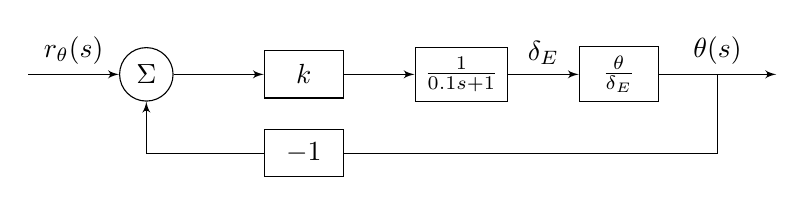
\begin{tikzpicture}[auto, node distance=2cm,>=latex']
            \node [input, name=input] {};
            \node [sum, right of=input, xshift=0.5cm] (sum) {$\Sigma$};
            \node [block, right of=sum] (controller) {$k$};
            \node [block, right of=controller] (actuator) {$\frac{1}{0.1s + 1}$};
            \node [block, right of=actuator] (plant) {$\frac{\theta}{\delta_E}$};
            \node [output, right of=plant] (output) {};
            \node [block, below of=controller, yshift=1cm] (feedback) {$-1$};
            
            \draw [draw,->] (input) -- node {$r_\theta(s)$} (sum);
            \draw [->] (sum) -- node {} (controller);
            \draw [->] (controller) -- node {} (actuator);
            \draw [->] (actuator) -- node {$\delta_E$} (plant);
            \draw [->] (plant) -- node [name=y] {$\theta(s)$}(output);
            \draw [-] (y) |- node [above,pos=0.79] {} (feedback);
            \draw [->] (feedback) -| node {} (sum);
        \end{tikzpicture}
    \end{center}
    \caption{Simple Proportional Controller with Feedback Loop}\label{fig}
\end{figure}

Applying finite value theorem to the closed loop error with step input gives
\begin{equation}
    \lim_{t \to \infty} e(t) = \lim_{s \to 0} s (r - \theta) = \lim_{s \to 0} \frac{1}{1+kH(s)G(s)} = \frac{K}{1+K} > 0.025
\end{equation}
For $G(s)$ as the fitted transfer function of elevator to pitch angle, and $H(s)$ as the first order elevator lag, the steady state error is given below.
\begin{equation}
    e_{ss} = \frac{0.07895}{0.07895 + 0.126421 k} < 0.025
\end{equation}
Which can be rearranged to give an lower bound on $k$ as $k > 24.36$.

\begin{figure}[H]
    \centering
    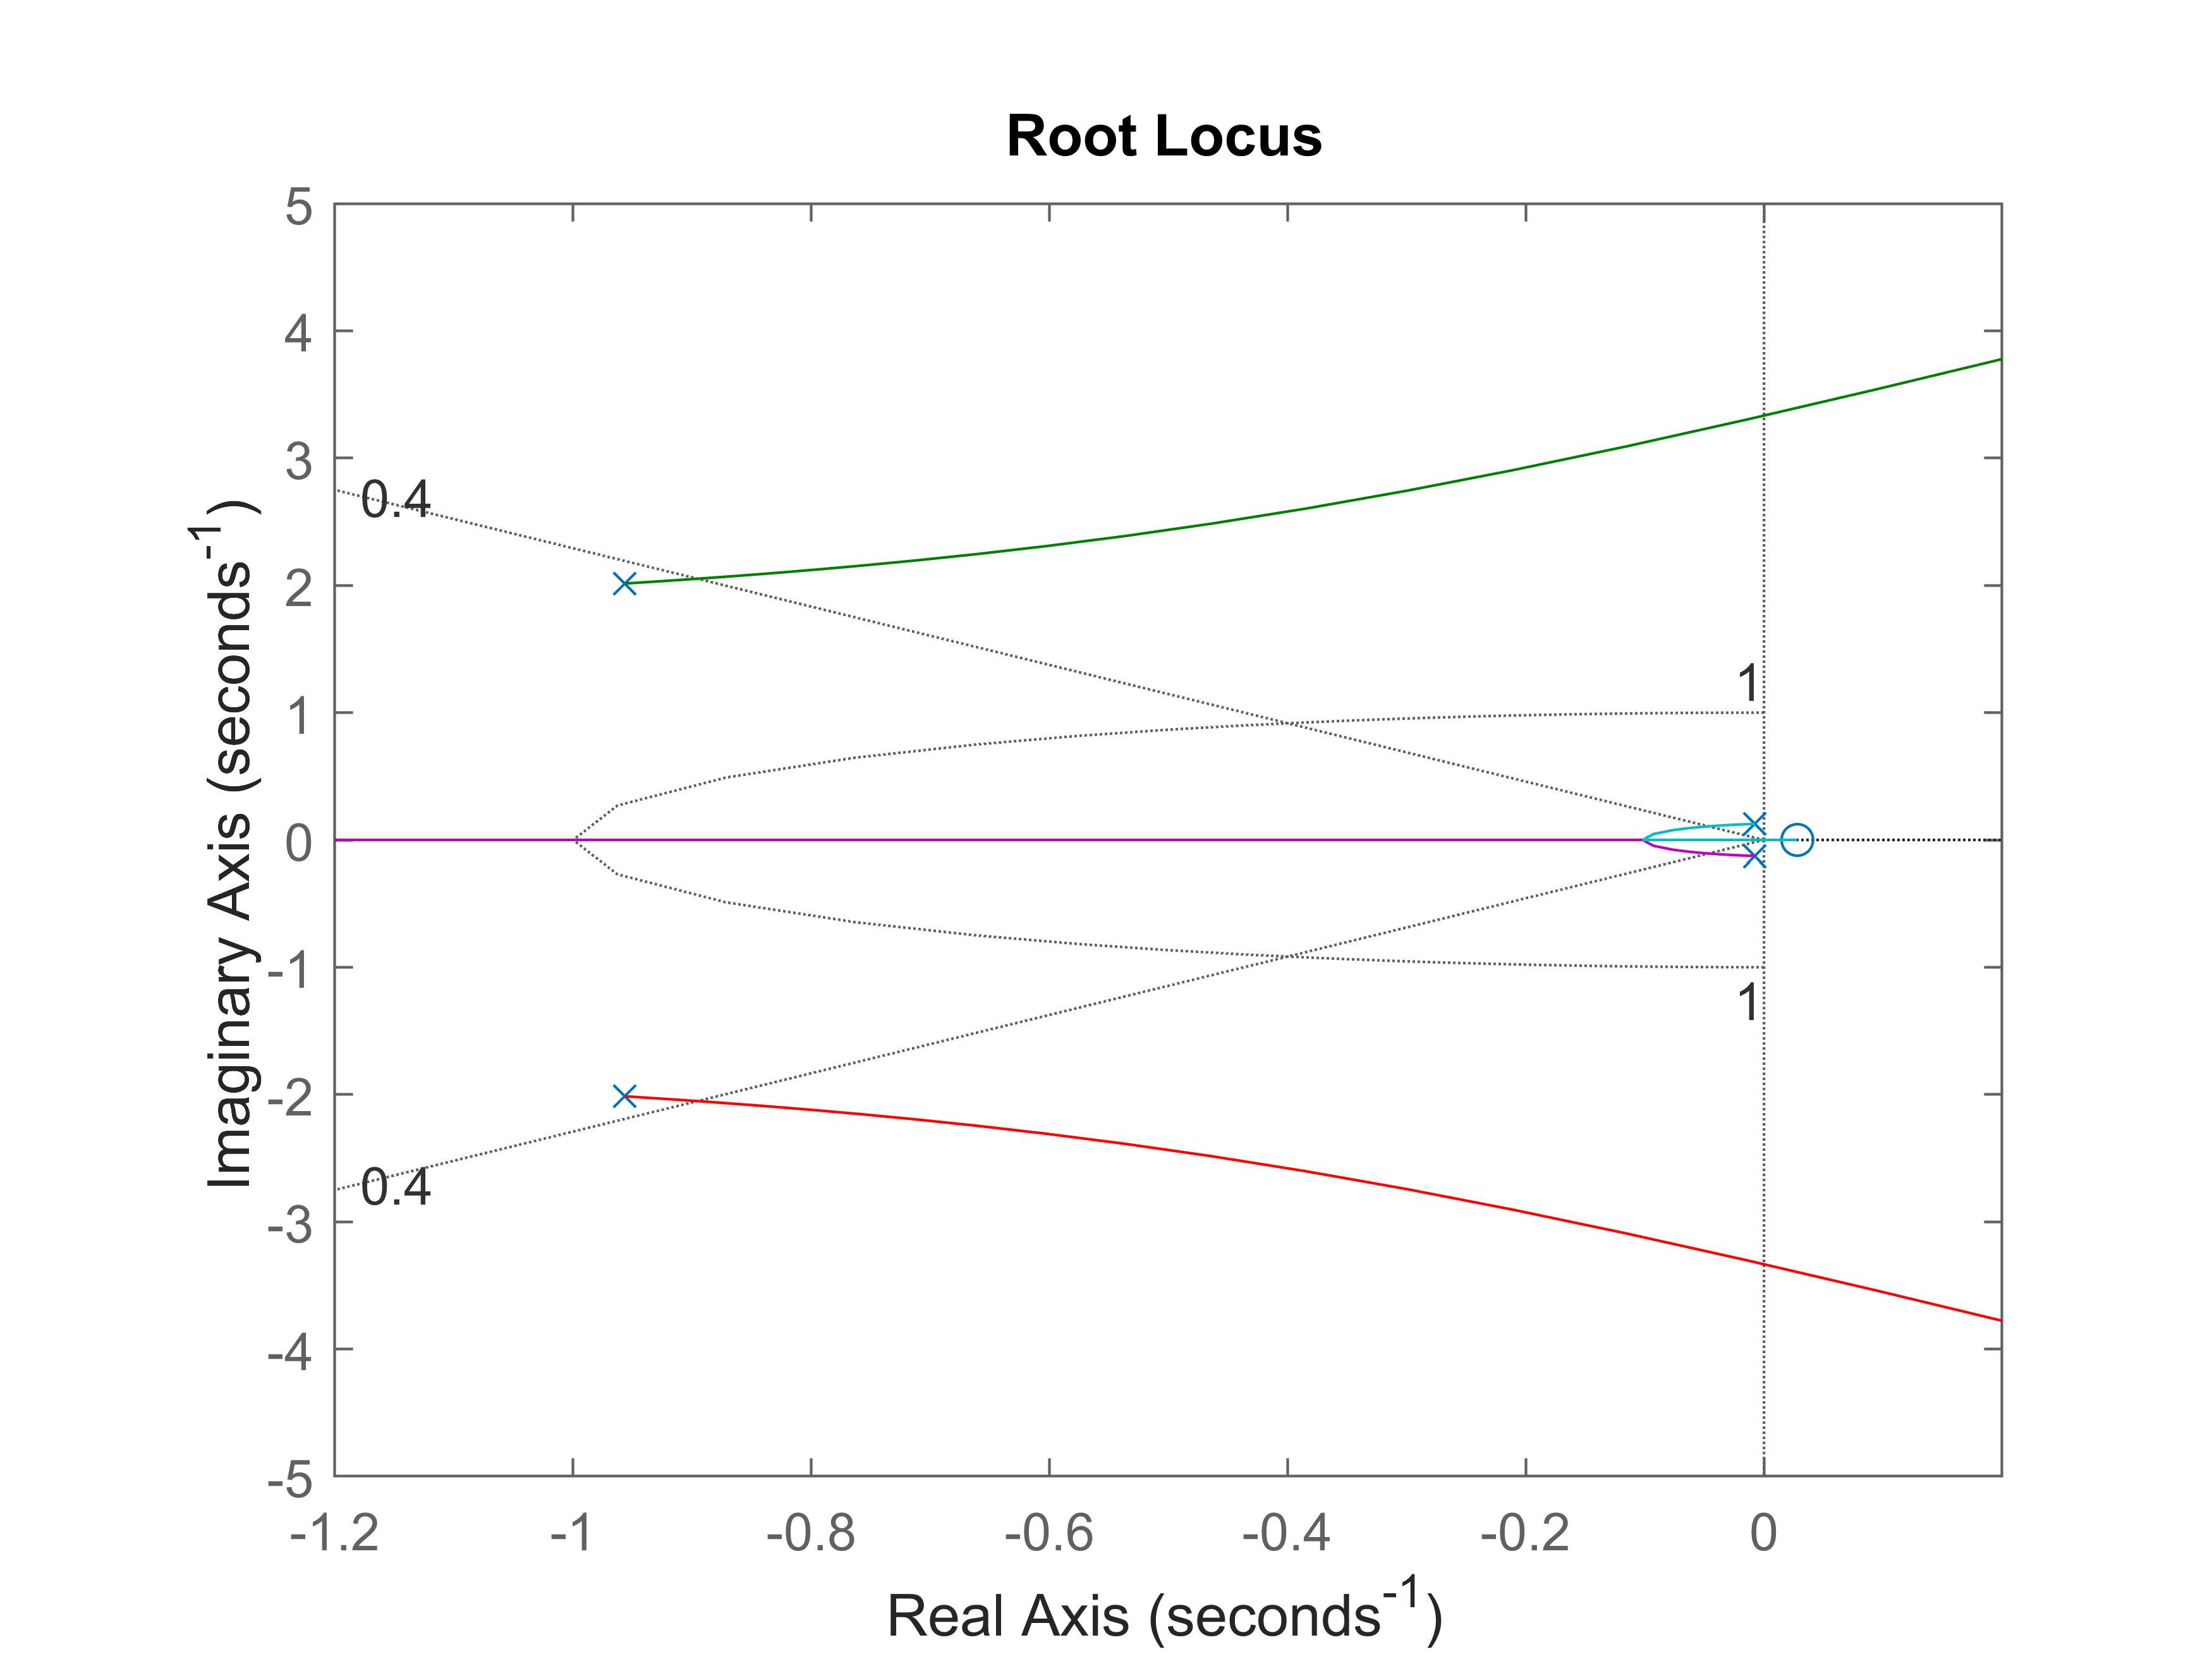
\includegraphics[width=0.6\textwidth]{figures/pitch_autopilot_locus_bad.png}
    \caption{Root locus of elevator servo and fitted pitch displacement transfer function.}
    \label{fig:fitted_pitchrate_rlocus}
\end{figure}

Figure \ref{fig:fitted_pitchrate_rlocus} shows the root locus for the fitted elevator to pitch angle transfer function shown in equation \ref{eq:pitch_elev}.
% TODO: explain the direction that the poles move as k increases and the tradeoff between SPO and phugoid damping.
For gain values $k>3.27$ the SPO poles move to the right half plane and so the system is unstable meaning the proportional controller is insufficient to meet both SPO damping and steady state error requirements.

The solution commonly used is to add an integrator to the controller which will completely eliminate steady state error.
This means replacing $k$ with $k(1 + \frac{1}{T_i s})$ in the controller block.
This will add a pole at $s=0$ and a zero at $s=-1/T_i$ to the root locus.

\begin{figure}[H]
    \centering
    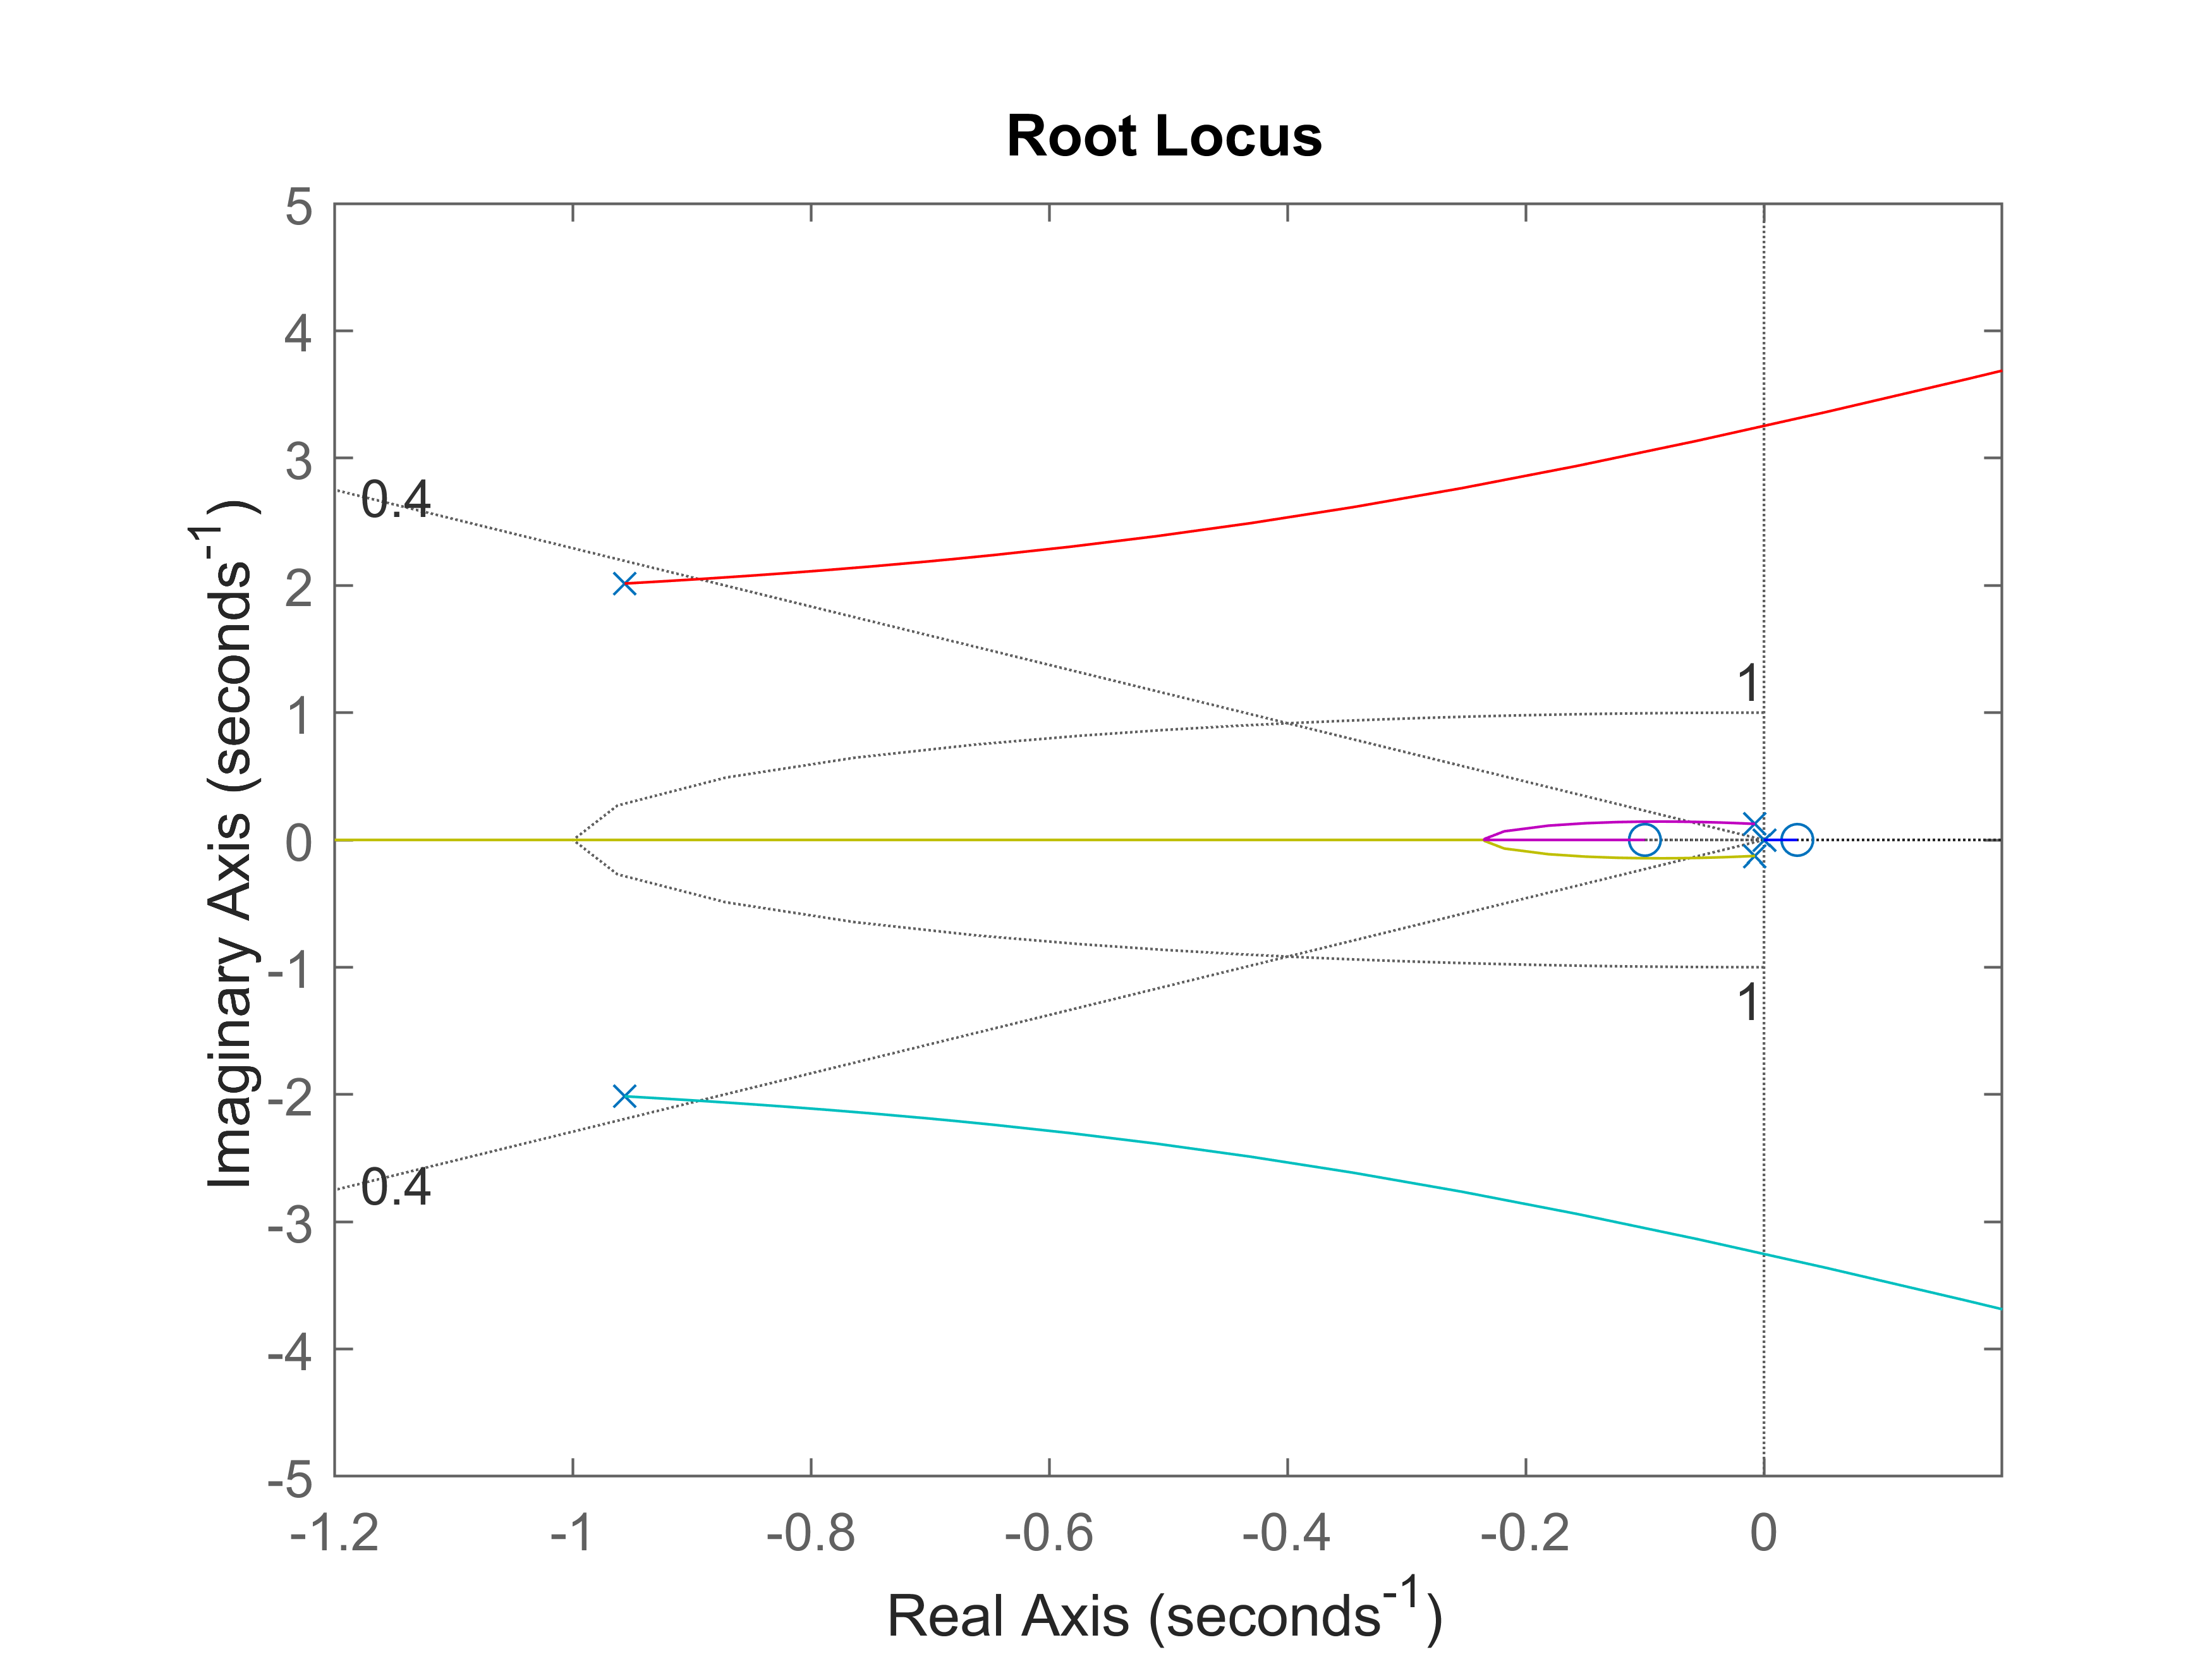
\includegraphics[width=0.6\textwidth]{figures/pitch_autopilot_locus_intbad.png}
    \caption{Root locus of elevator servo and fitted pitch displacement transfer function with added integrator time constant $T_i = 10$.}
    \label{fig:fitted_pitchrate_rlocus_int}
\end{figure}

Figure \ref{fig:fitted_pitchrate_rlocus_int} shows the fitted elevator to pitch angle root locus with an integrator time constant $T_i = 10$.
As expected there is a zero at $s=-0.1$ and a pole at $s=0$.
However the existence of the zero in the RHP and the new integrator pole at 0, right of the phugoid poles, causes the region on the real axis between the zero and pole to be on the root locus.
This causes the closed loop to be unstable for all gain values.

Comparison to representative transfer functions \cite{rep} shows the final term on the numerator of my fitted transfer function to have the opposite sign.
It was then decided to use the representative transfer function for the elevator to pitch angle from this point onwards.

\begin{figure}[H]
    \centering
    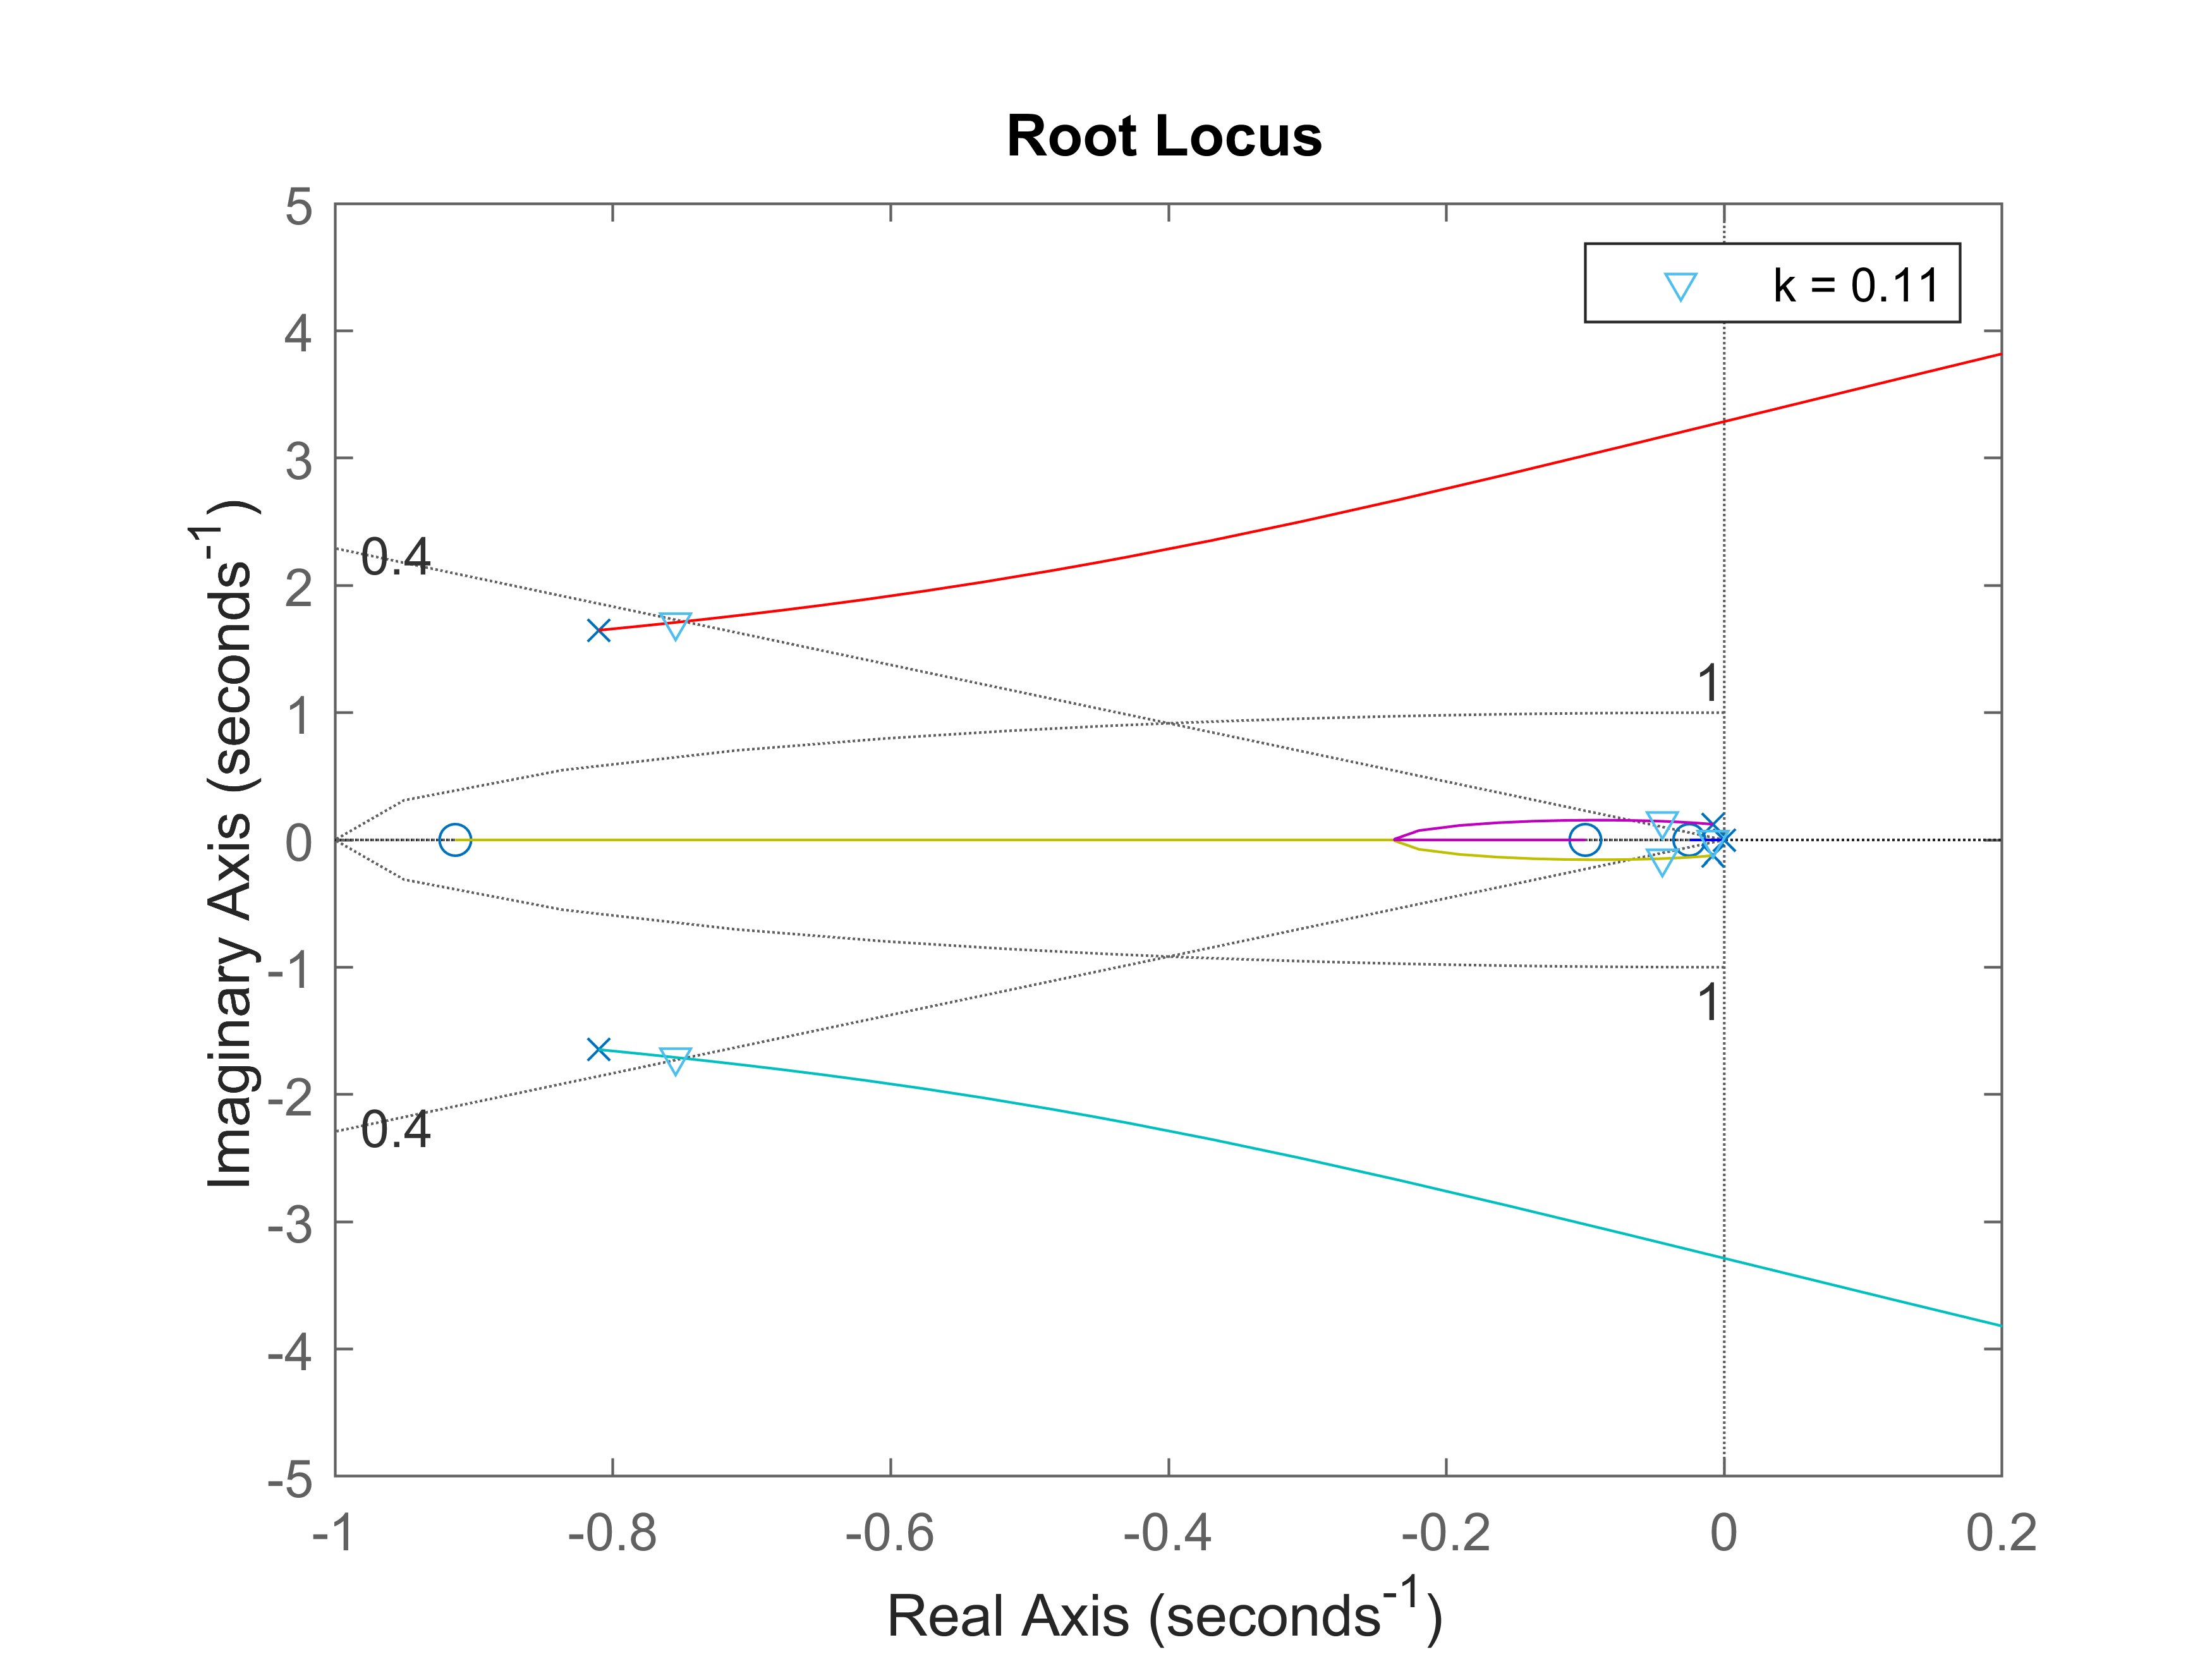
\includegraphics[width=0.6\textwidth]{figures/pitch_autopilot_locus_Ti.png}
    \caption{Root locus of elevator servo and representative pitch transfer function \cite{rep} with added integrator time constant $T_i = 10$.}
    \label{fig:representative_pitchrate_rlocus_int}
\end{figure}

Figure \ref{fig:representative_pitchrate_rlocus_int} shows the root locus for the representative elevator to pitch angle transfer function.
The pole can now be seen to lie in the LHP for all gain values and is stable.
The SPO poles can be seen to only have a narrow window of gain values $k < 0.12$ that satisfy the damping ratio requirement shown by the dotted line.

\begin{figure}[H]
    \centering
    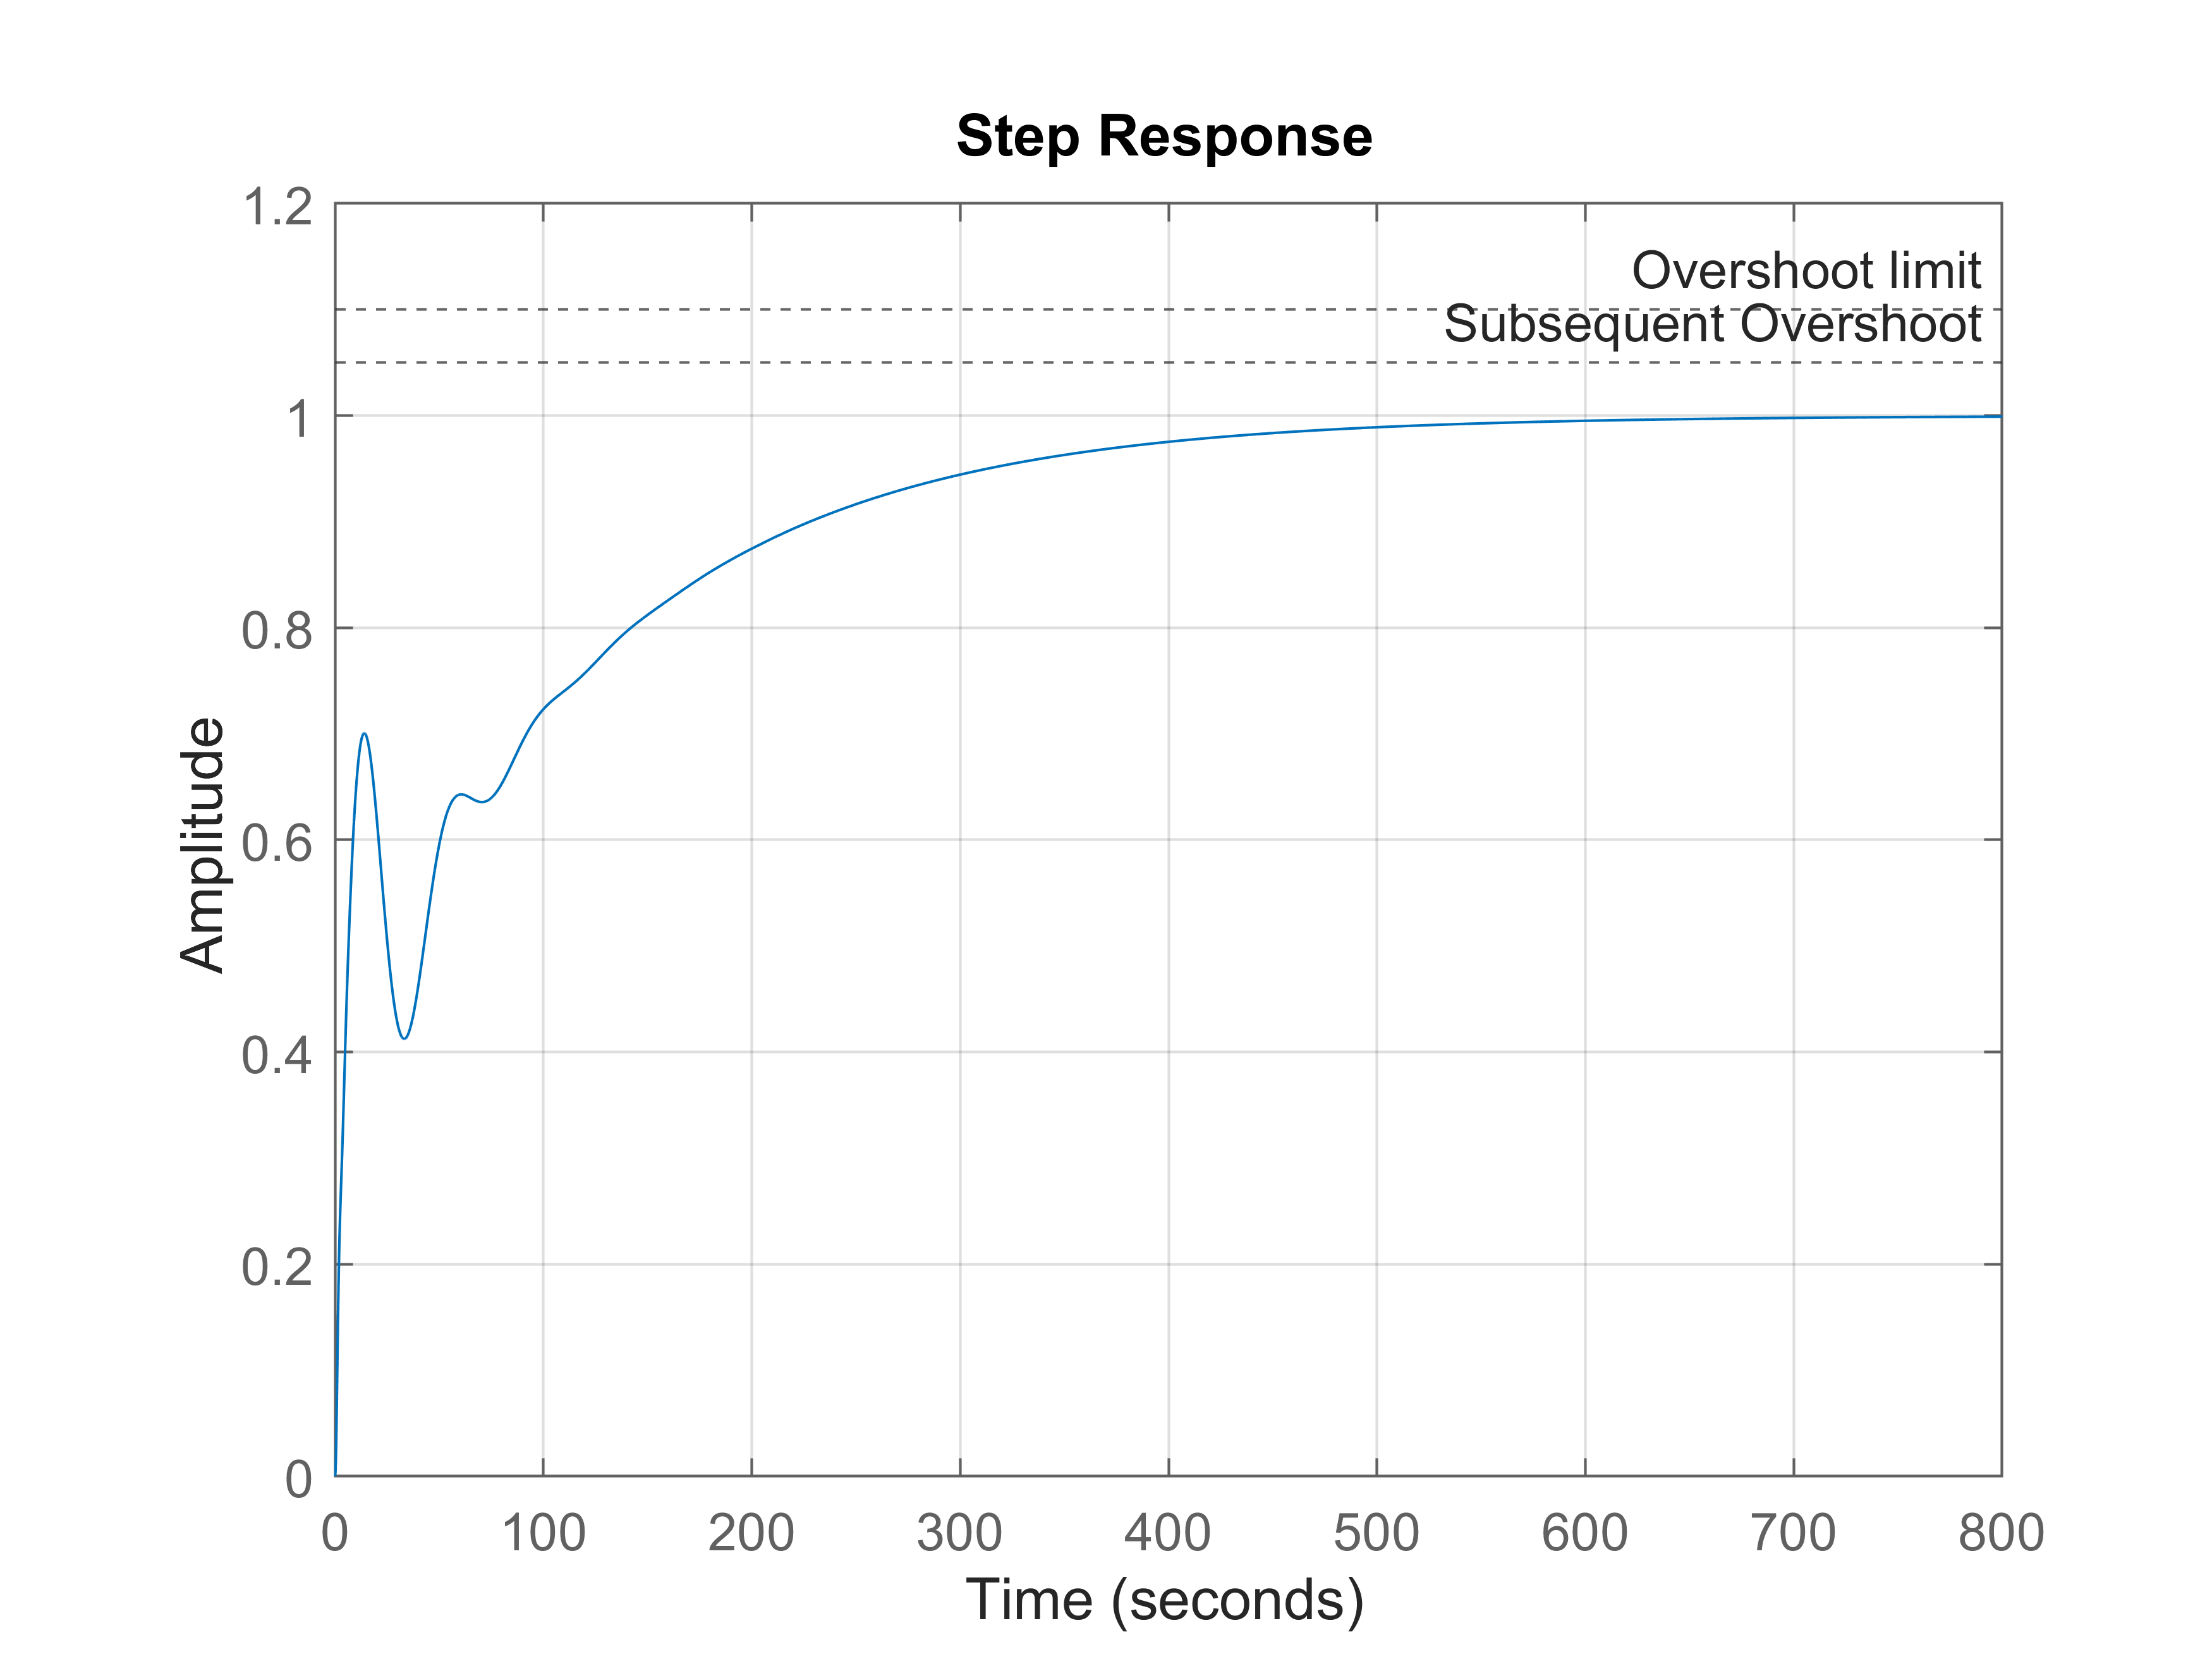
\includegraphics[width=0.6\textwidth]{figures/pitch_autopilot_uncompensated_step.png}
    \caption{Step response of PI controlled pitch displacement with $k=0.11$ and $T_i = 10$.}
    \label{fig:pitch_autopilot_uncompensated_step}
\end{figure}

Figure shows the step response for the PI controlled pitch displacement with $k=0.11$ and $T_i = 10$.
While the response technically meets the requirements as it doesn't overshoot, a settling time of 226 seconds is far too slow in practice.
A higher gain must be used but this decreases the SPO damping and so to meet the requirements and have a fast response a more complex controller must be used.

To increase damping ratio, an additional component of derivative is often used.
Another option is a more general form called a phase lead compensator.
For the most simple controller, a derivative term was added to the controller block making it:
\begin{equation}
    k\left(1 + \frac{1}{T_i s} + T_d s\right)
\end{equation}

\begin{figure}[H]
    \centering
    \begin{subfigure}{0.45\textwidth}
        \centering
        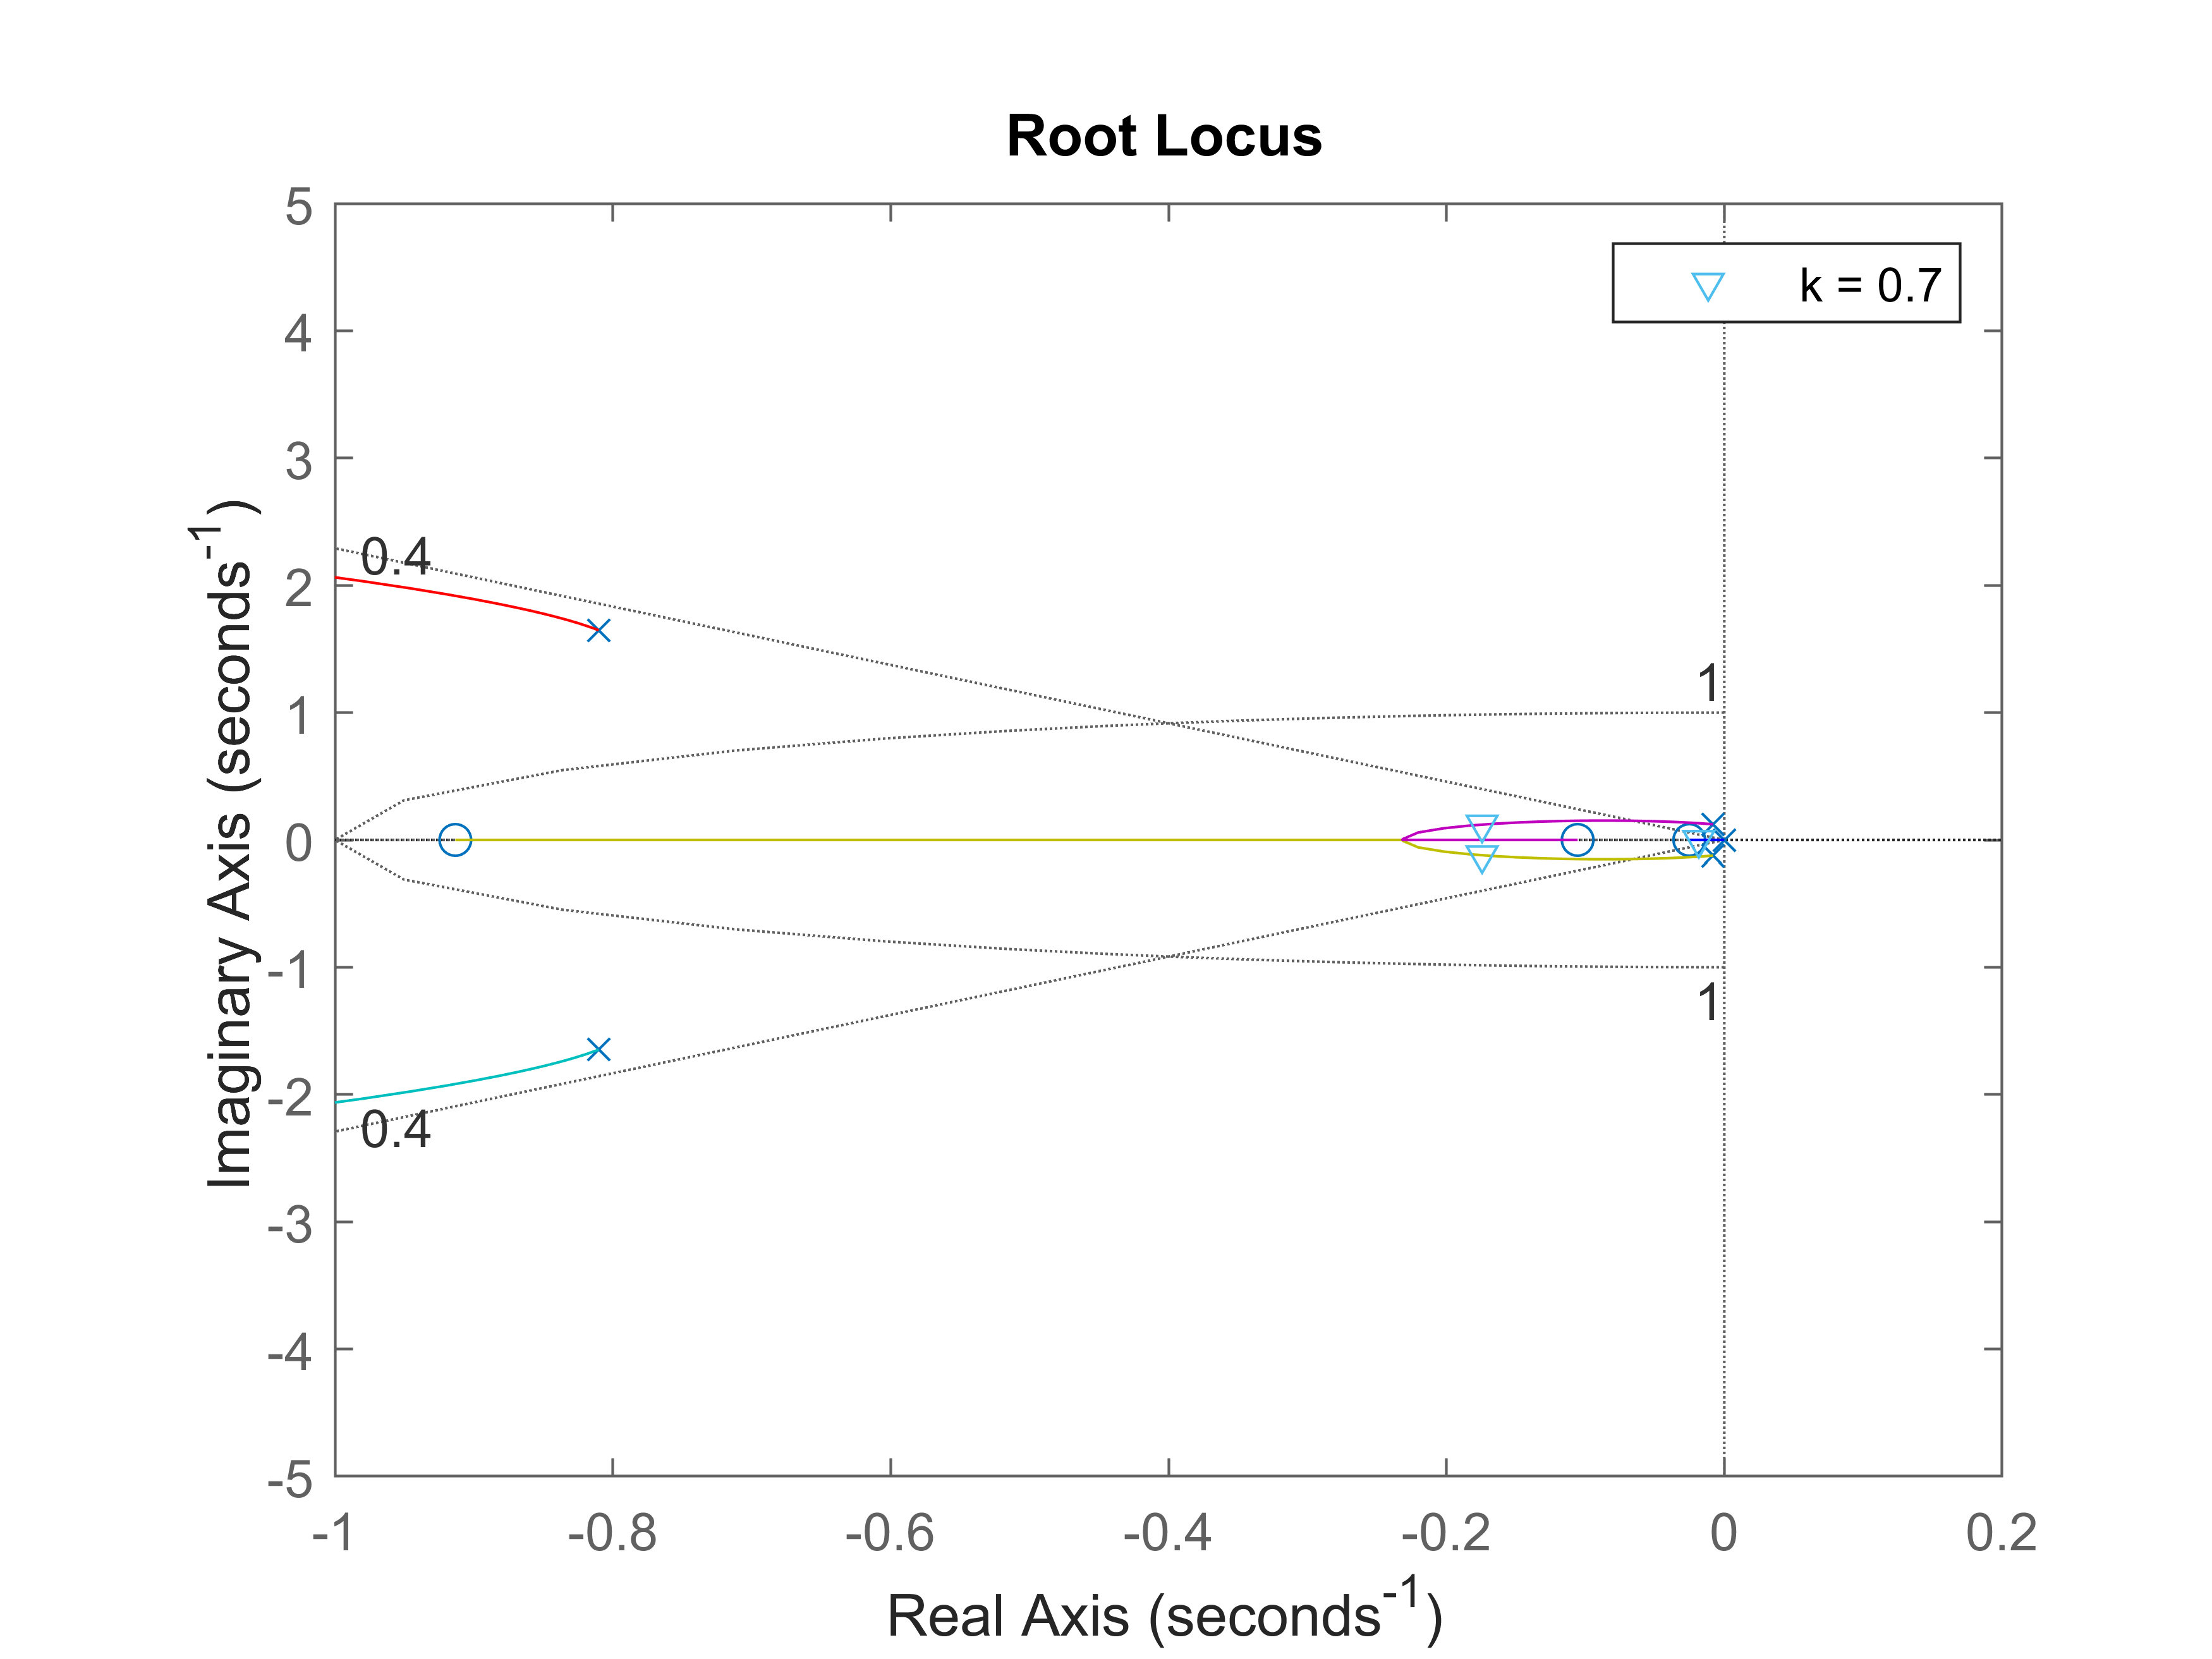
\includegraphics[width=0.99\textwidth]{figures/pitch_autopilot_locus_TiTd.png}
    \end{subfigure}
    \begin{subfigure}{0.45\textwidth}
        \centering
        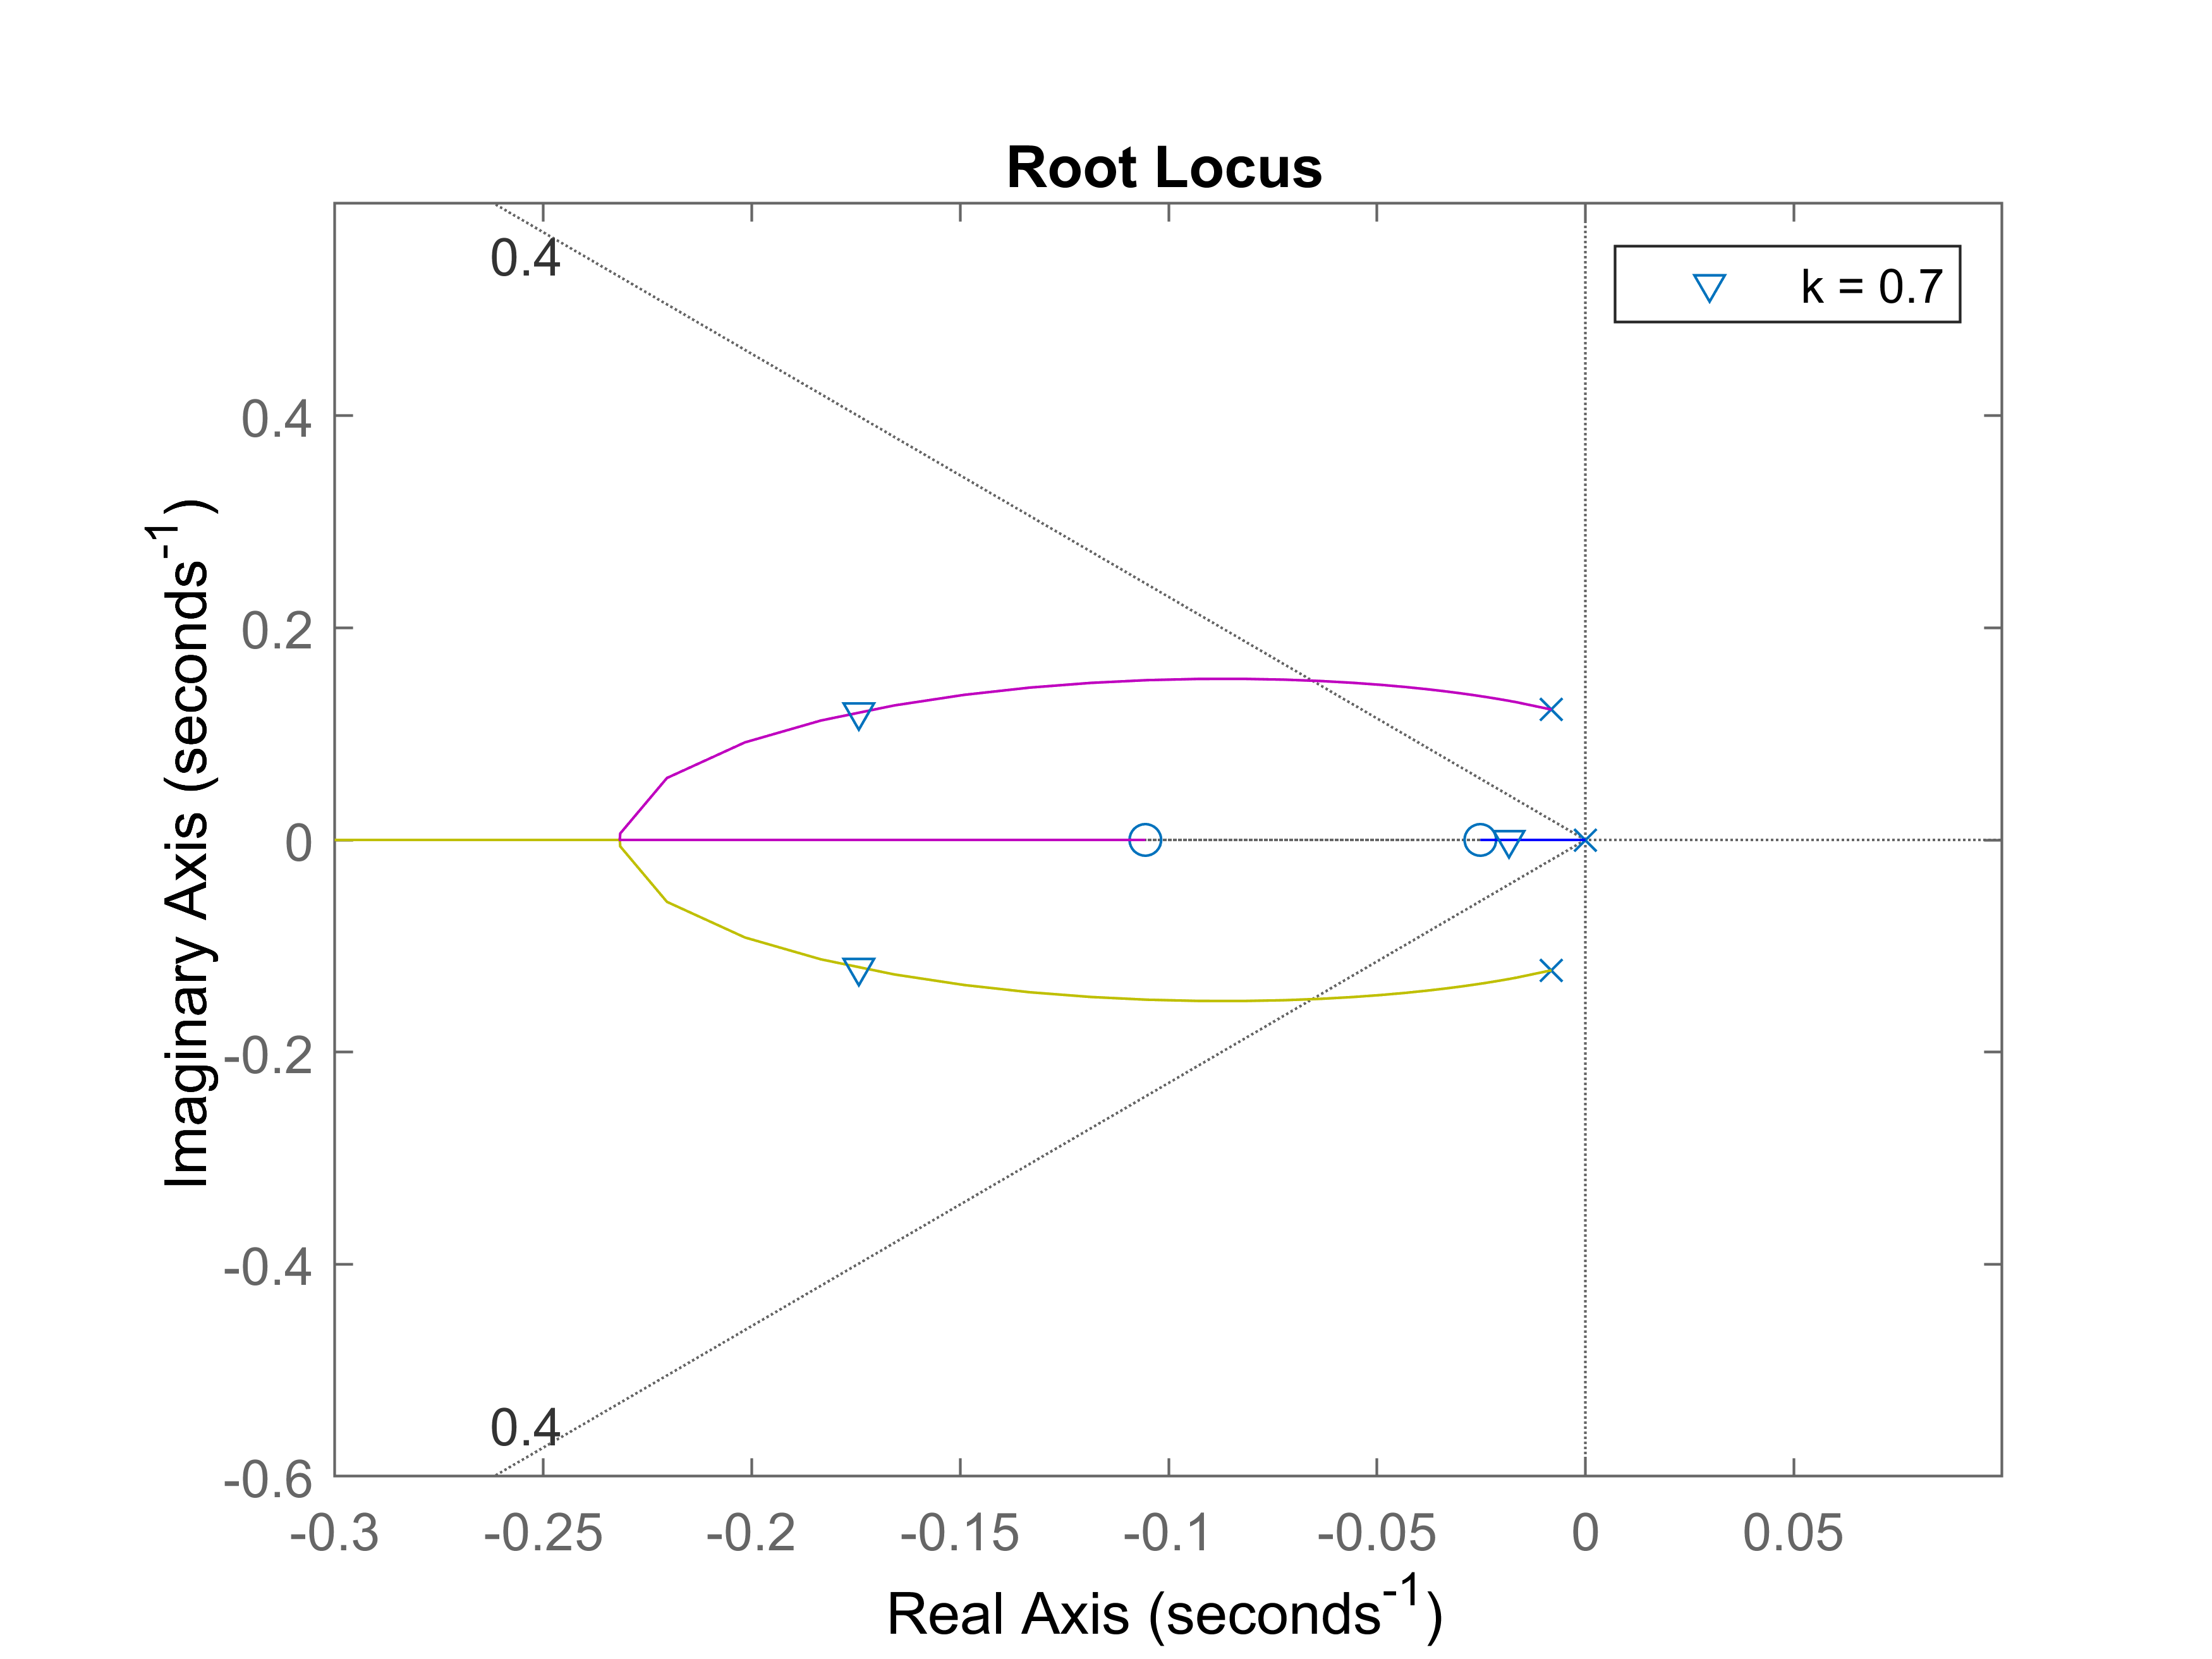
\includegraphics[width=0.99\textwidth]{figures/pitch_autopilot_locus_TiTd_zoomed.png}
    \end{subfigure}
    \caption{Root locus of elevator servo and representative pitch transfer function \cite{rep} with added integrator and derivative terms of time constants $10$, $0.5$ respectively.}
    \label{fig:pitch_autopilot_compensated_locus}
\end{figure}

\begin{figure}[H]
    \centering
    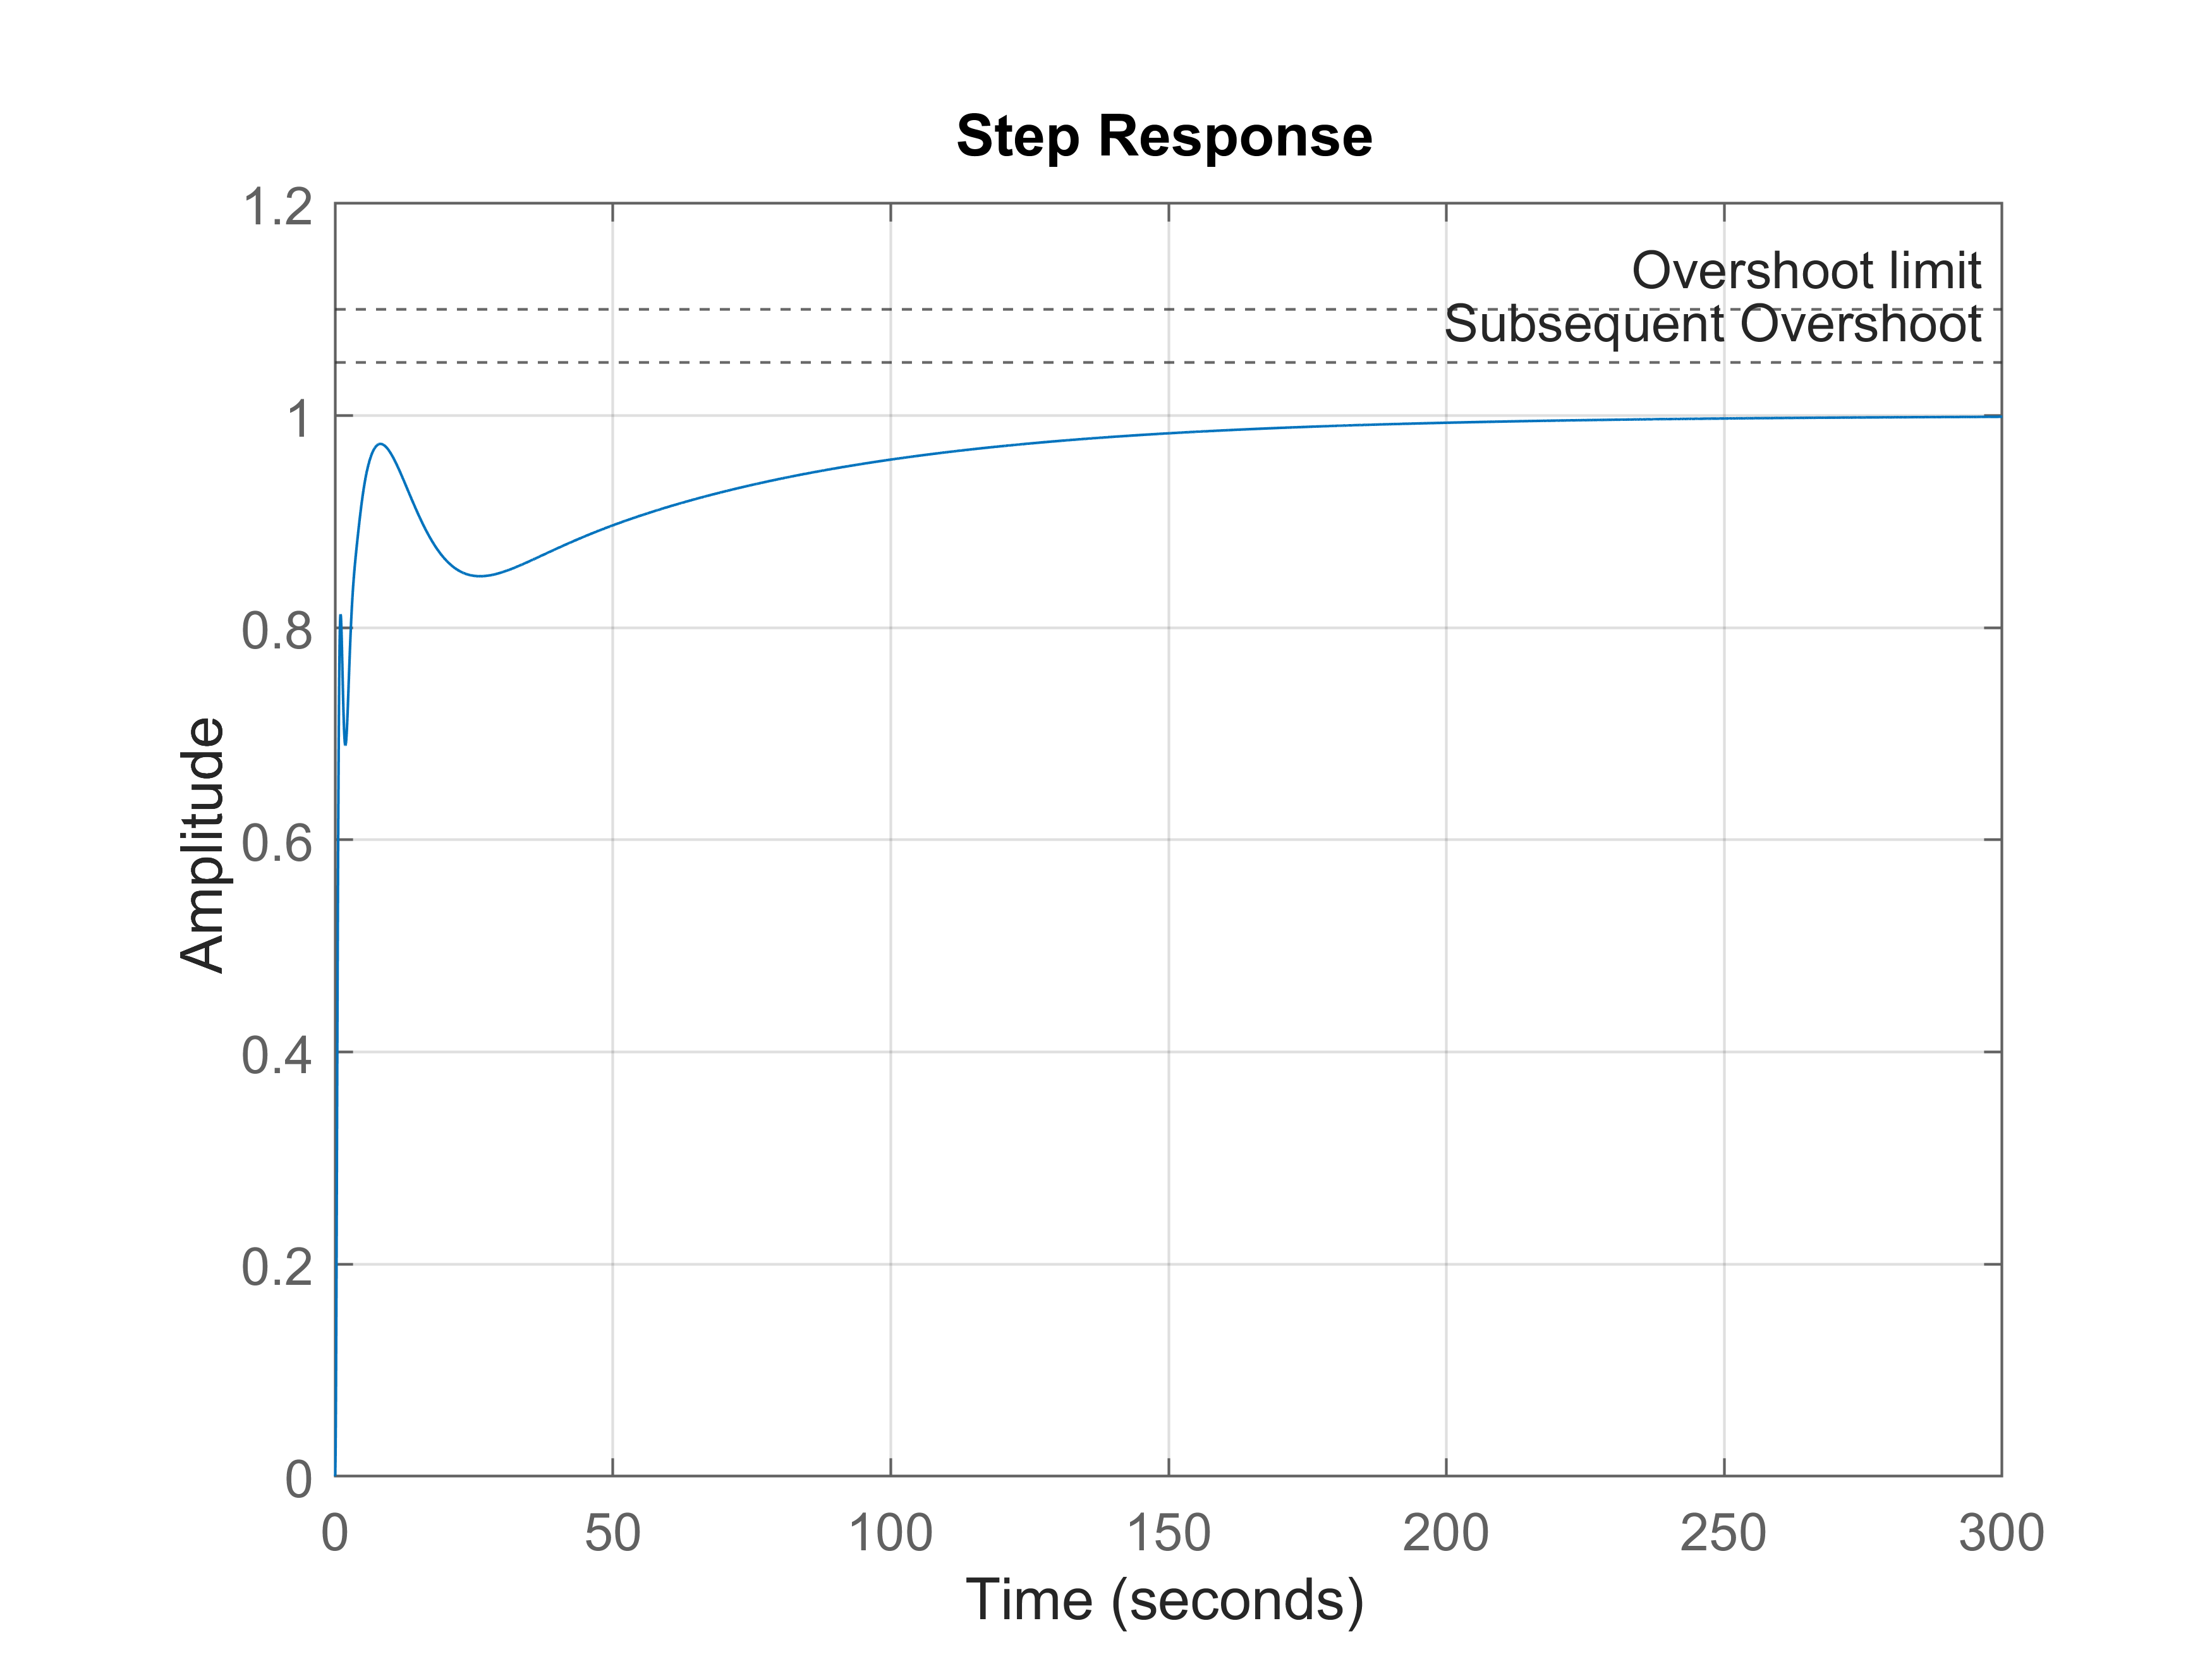
\includegraphics[width=0.6\textwidth]{figures/pitch_autopilot_compensated_step.png}
    \caption{Step response of PID controller with $k=0.70$, $T_i = 10$ and $T_d = 0.5$.}
    \label{fig:pitch_autopilot_compensated_step}
\end{figure}

Figure \ref{fig:pitch_autopilot_compensated_step} shows the step response of the PID controlled pitch displacement with $k=0.70$, $T_i = 10$ and $T_d = 0.5$.
Again it can be seen for small gains, increasing gain increases SPO damping, until a point where it decreases and then rapidly decreases before they become unstable.
At the same time increasing the gain from small values increases the phugoid damping ratio.
A tradeoff is found at the maximum damping ratio of the SPO mode which is the dominant mode in the initial transience of the step response.
The damping ratio of the phugoid mode is still very high here at 0.83 and all the other requirements are satisfied.
If lower frequency disturbances, perhaps in the form of gusts, are expected, then a higher gain may be more suitable to increase the phugoid damping ratio,
at the cost of performance at higher frequency disturbances close to the SPO mode.

\subsubsection{Autotuning of Pitch Displacement}

The most simple form of controller identified to meet the requirements was a PID controller, for which
there exists many rule based autotuning methods \cite{autotune}.
Three methods were peformed and their step responses can be seen in figure \ref{fig:pitch_autopilot_autotune_step} below.

\begin{figure}[H]
    \centering
    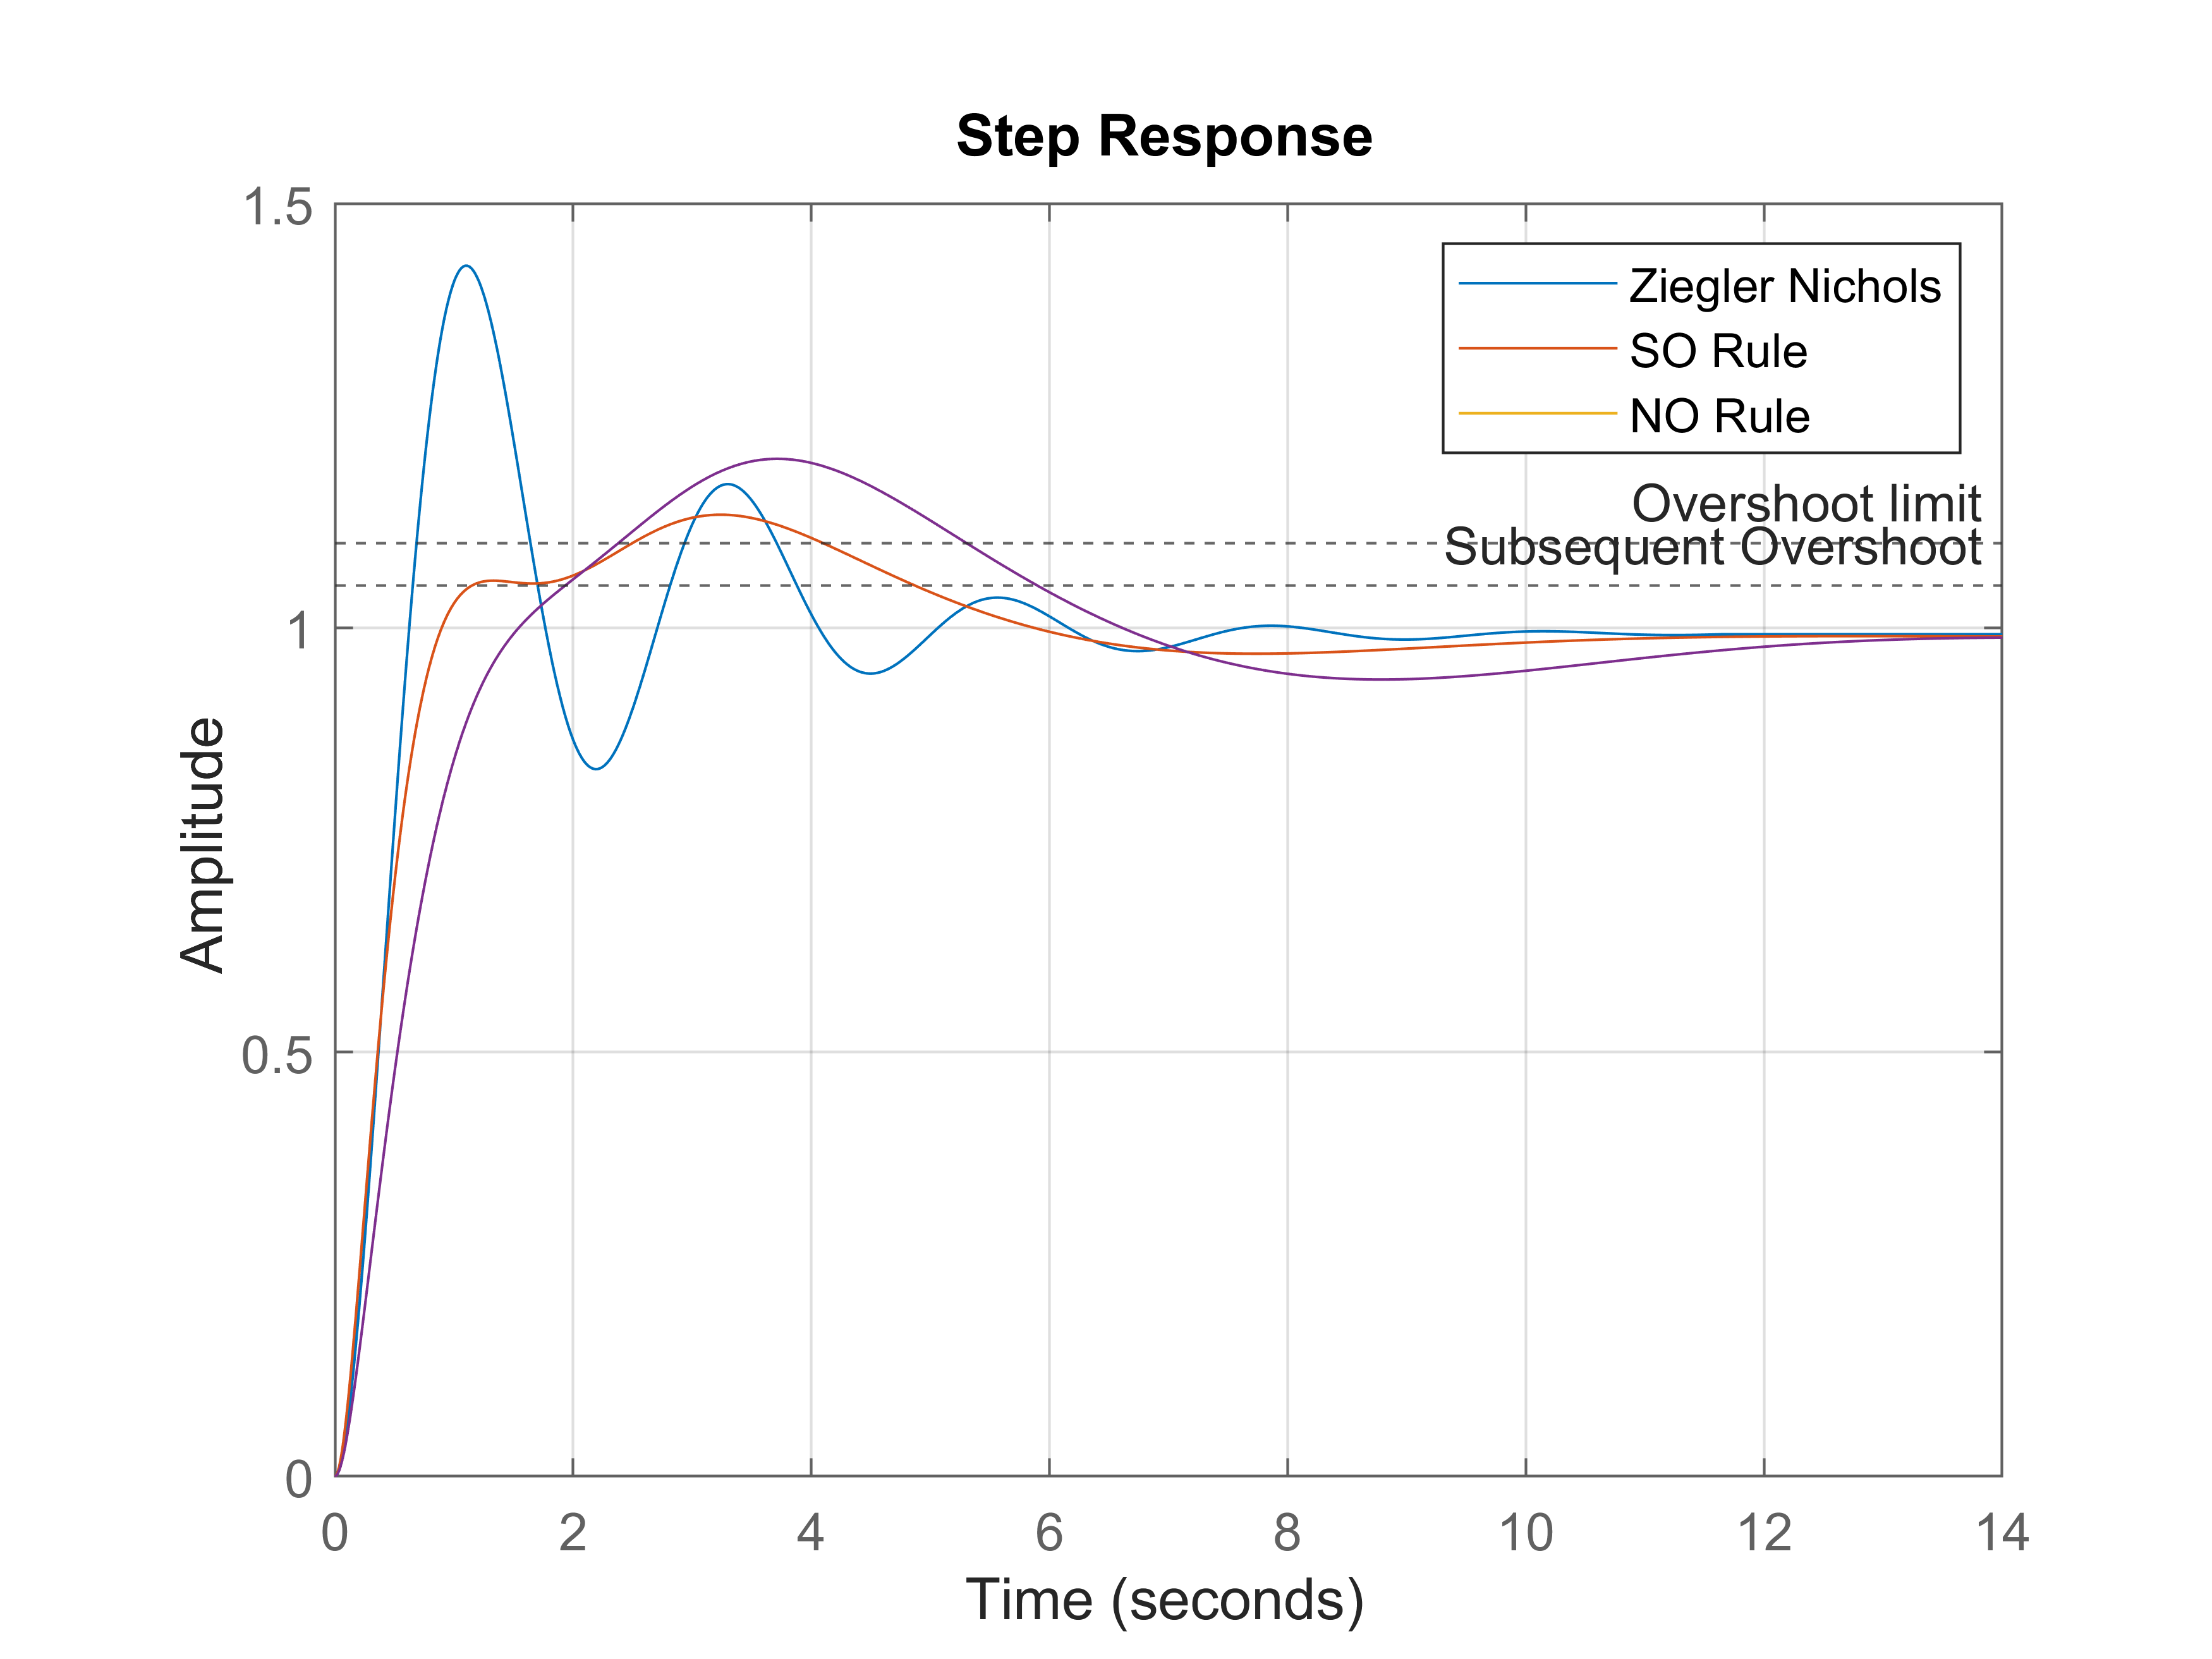
\includegraphics[width=0.6\textwidth]{figures/pitch_autopilot_autotuning_comparison.png}
    \caption{Step response of PID controlled pitch displacement with autotuned parameters. NO - No overshoot, SO - Some overshoot.}
    \label{fig:pitch_autopilot_autotune_step}
\end{figure}

With little information about the system, only the frequency and gain value at which the SPO pole becomes unstable, the autotuning methods were able to find functional controllers.
The performance does not meet the requirements for overshoot or in the Ziegler Nichols case the damping requirements.
The some overshoot suprisingly had less overshoot than the no overshoot method, although this was due to a different mode, the phugoid, being dominant in the response.
This is inherently due to the methods being more applicable to lower order systems.
However, given the simplicity of the rule based methods, they could provide an initial guess for the controller parameters to be numerically optimised.
Such optimisation would require a cost function to be defined which could be an integrated absolute error or a weighted sum of the overshoot and settling time properties \ref{fig:matlab_step_chics}.
% TODO: explain differences between the three methods
% None of which met the overshoot requirement explain why.

\subsection{Roll displacement autopilot}

\begin{figure}[H]
    \centering
    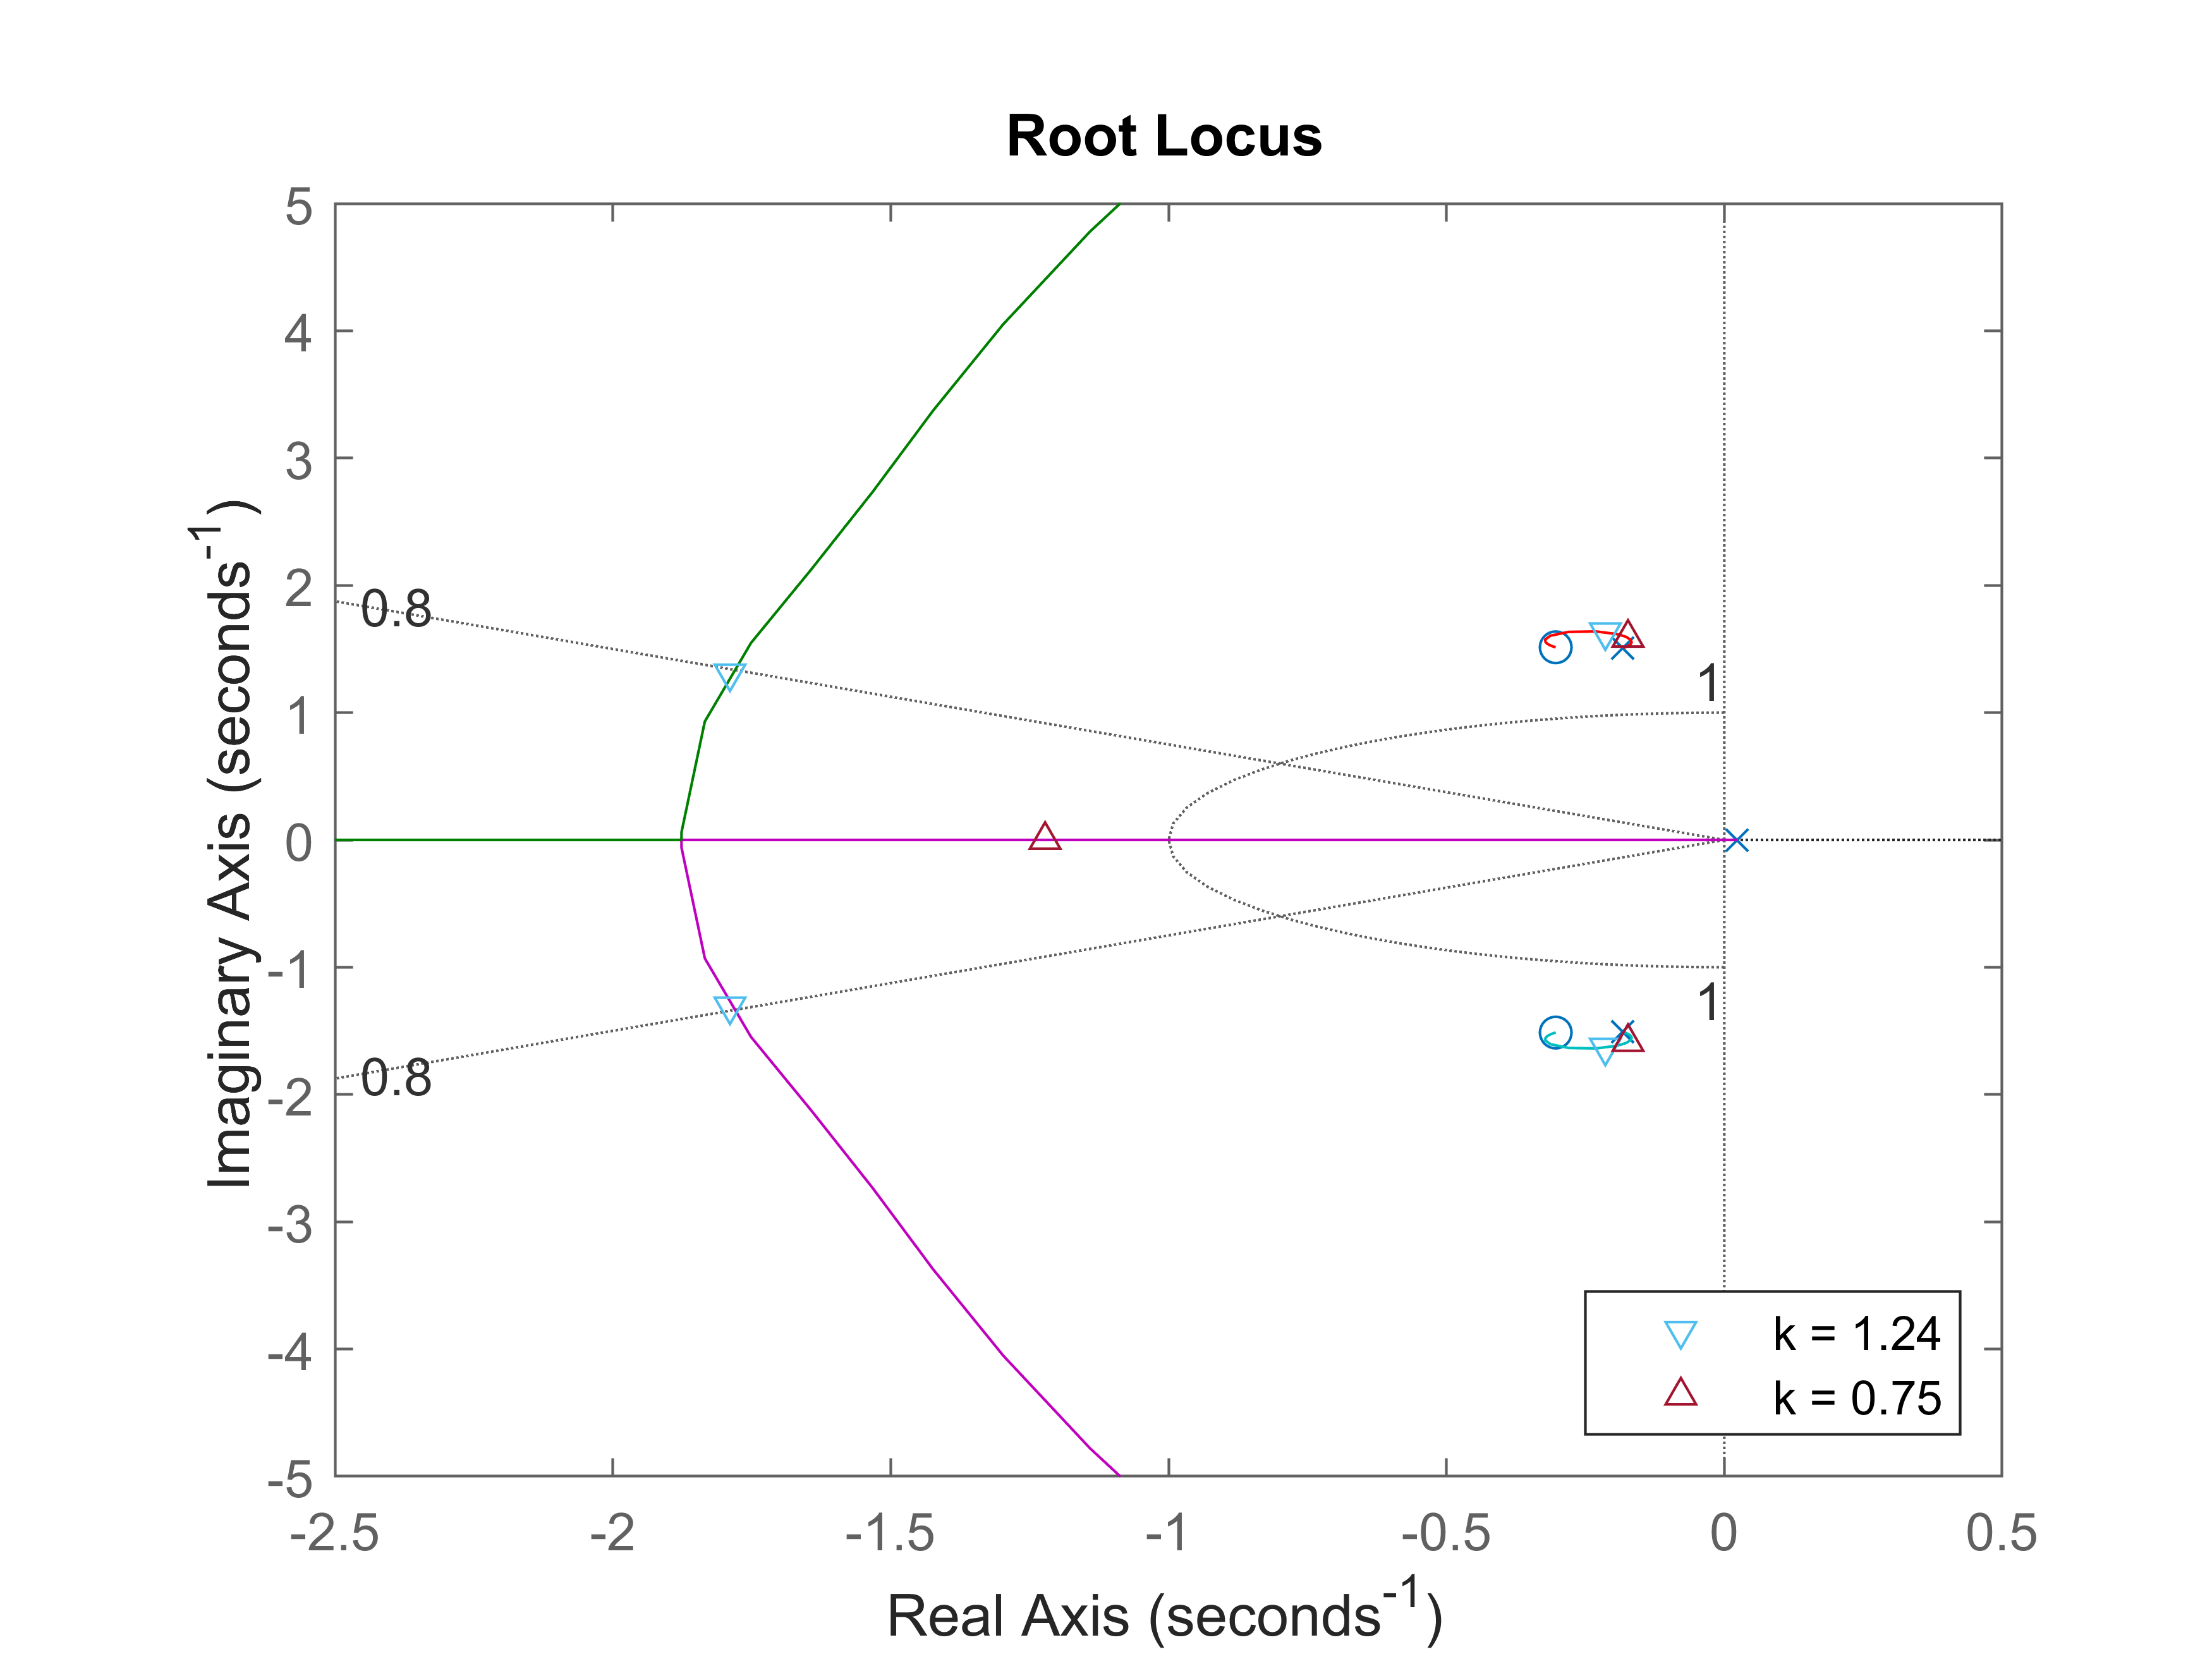
\includegraphics[width=0.6\textwidth]{figures/roll_autopilot_locus_uncompensated.png}
    \caption{Root locus of aileron servo and fitted roll displacement transfer function}
    \label{fig:roll_autopilot_uncompensated_locus}
\end{figure}

The root locus of fitted roll displacement transfer function can be seen above in figure \ref{fig:roll_autopilot_uncompensated_locus}.
The oscillatory dutch roll poles can be seen to move towards a pair of zeros within a small region of low damping.
The only requirement for this though is stability which is satisfied for all gain values.
The spiral mode pole is initially unstable, lying in the RHP, but moves to the LHP for gain values $k > 0.02$.
Interestingly the spiral and roll subsidence poles merge and become a complex conjugate pair for $k > 0.85$.
% TODO: physical interpretation of this?

\begin{figure}[H]
    \centering
    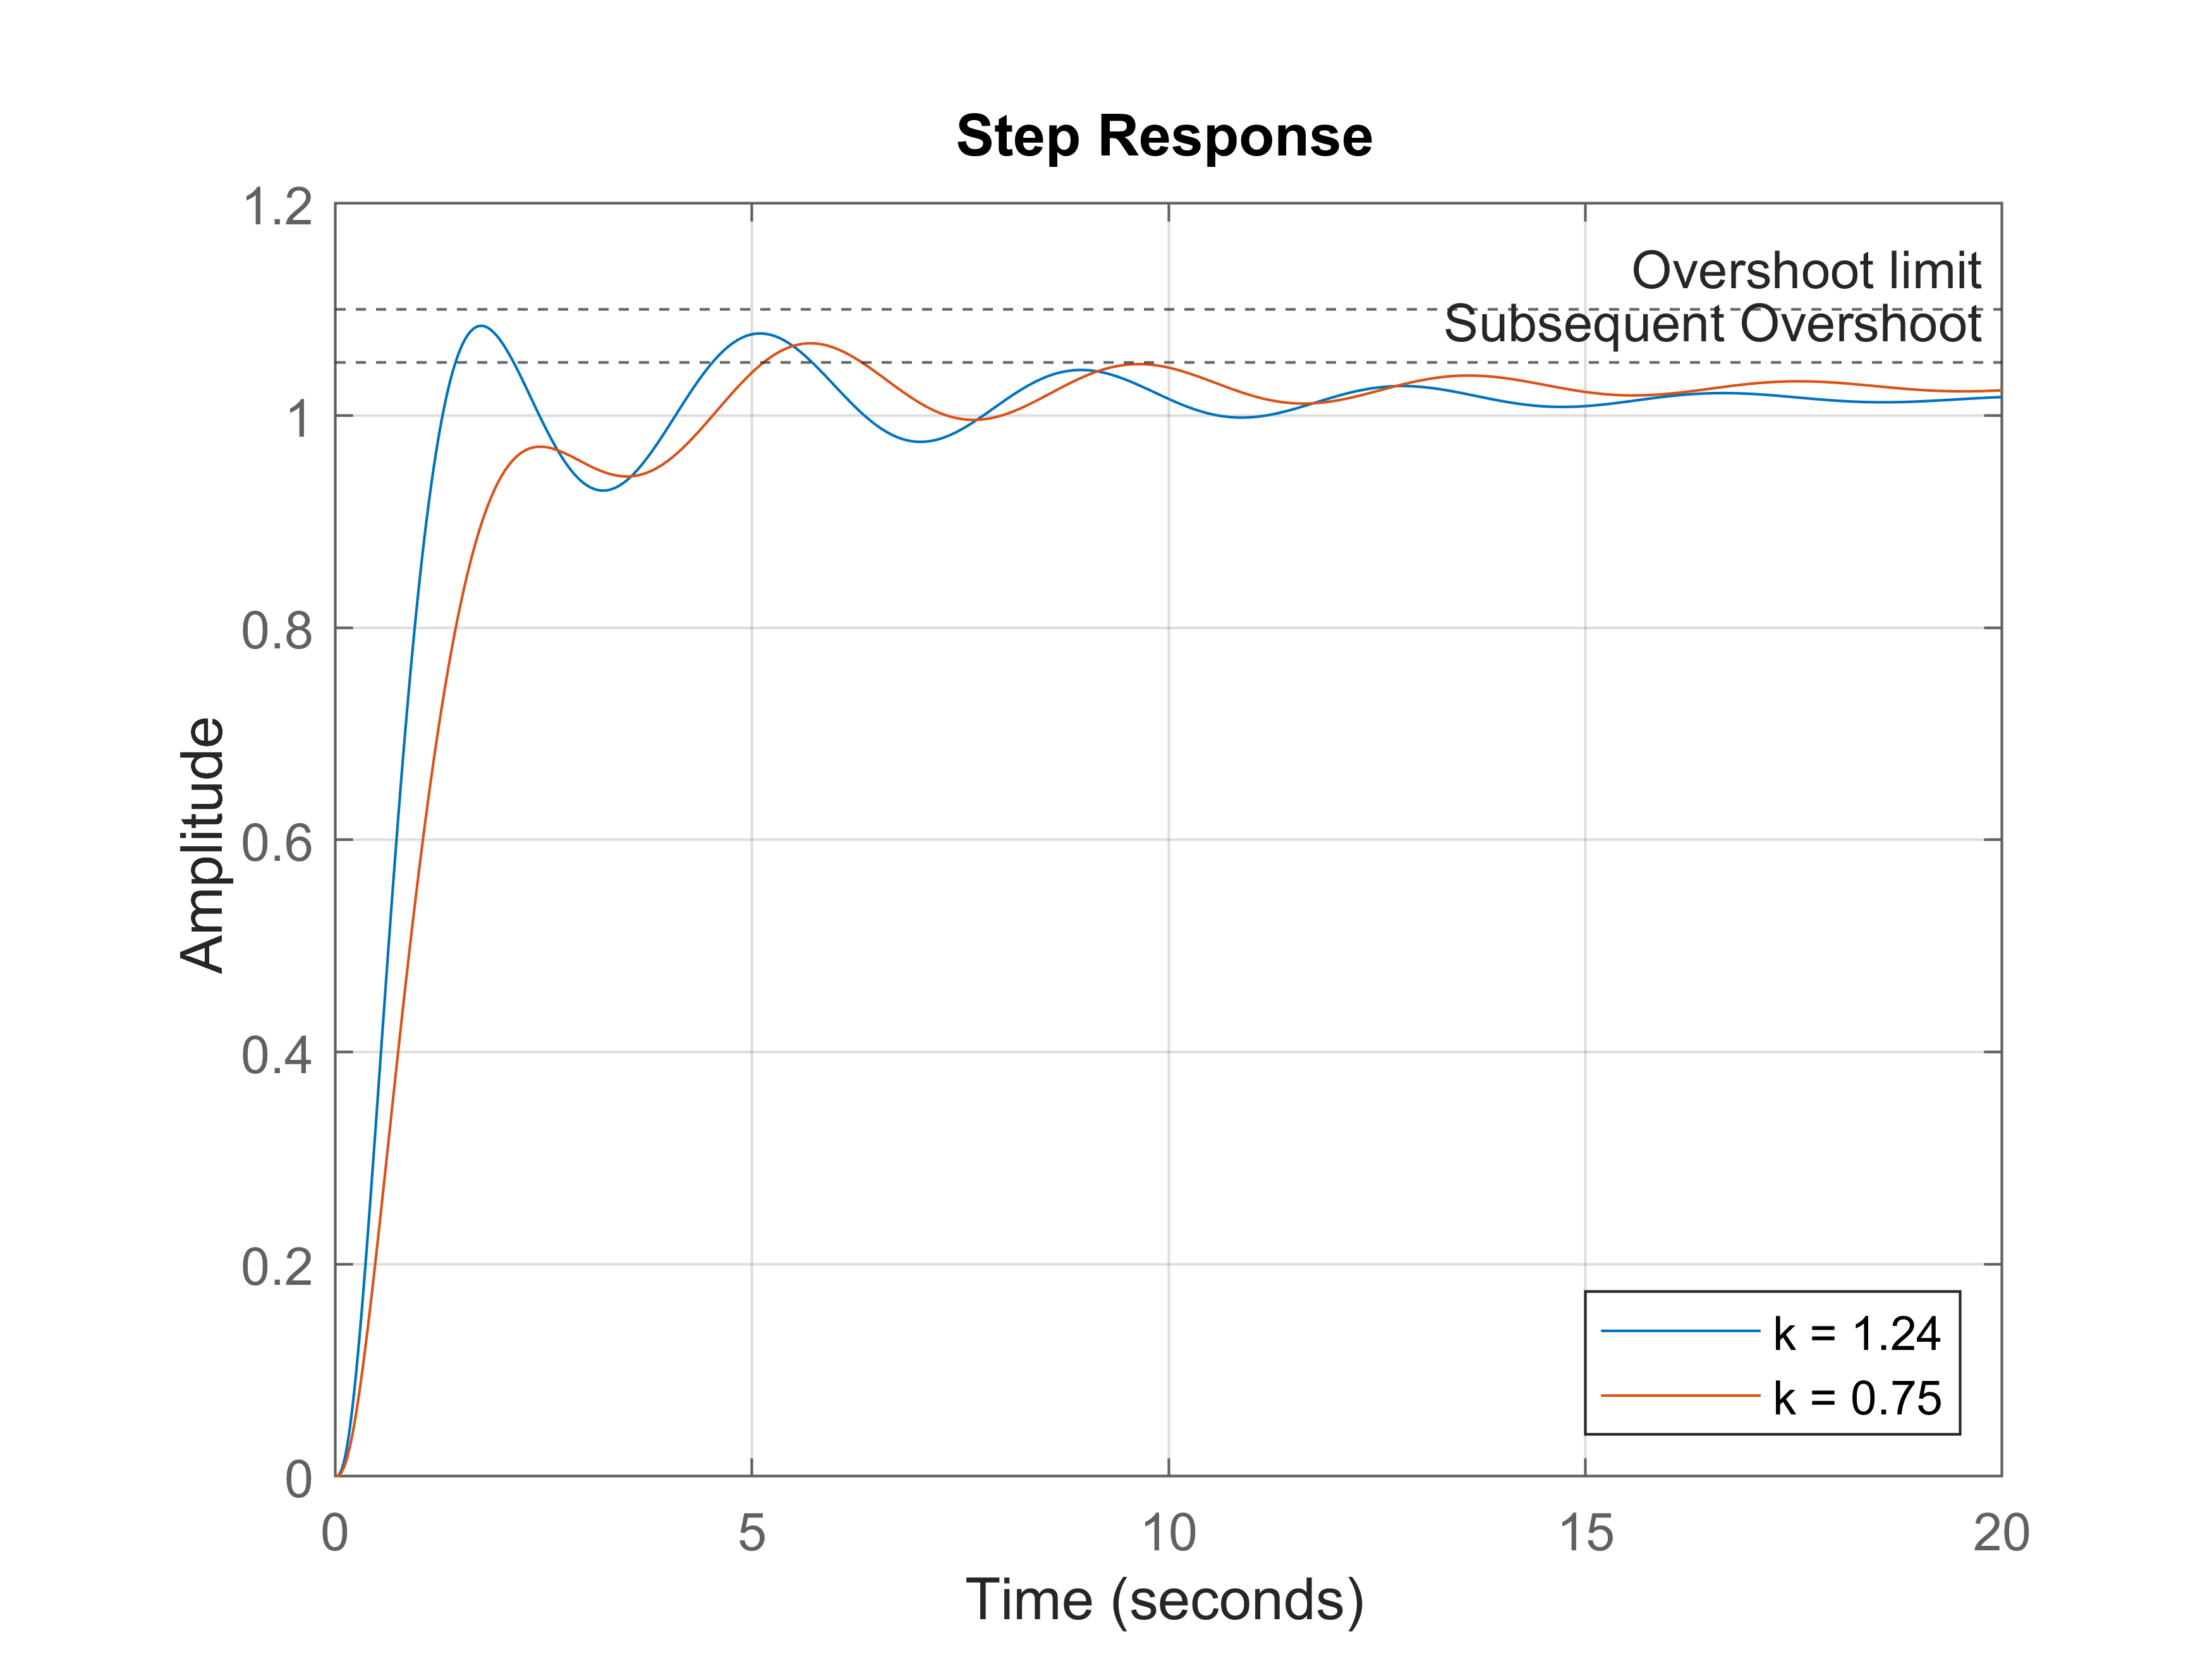
\includegraphics[width=0.6\textwidth]{figures/roll_autopilot_step_uncompensated.png}
    \caption{}
    \label{fig:roll_autopilot_step_uncompensated}
\end{figure}

Figure \ref{fig:roll_autopilot_step_uncompensated} shows the closed loop step responses for the gain values shown in figure \ref{fig:roll_autopilot_uncompensated_locus}.
The requirement for the subsequent oscillations to be $5 \%$ of the steady state is more strict than the oscillatory mode damping ratio requirement $\zeta_{RS}<0.8$.
The gain nearest to this damping limit is $k=1.24$ but the value of $k=0.75$ was found to satisfy the requirement whilst still having a fast response.
The spiral and roll subsidence poles are non-oscillatory for this value but satisfy the relevent requirements \ref{req:RS}.
At smaller gain values the dutch roll damping and roll subsidence time constant decreases which is not desirable.

While this controller meets the criteria, an additional complexity in the form of a derivative term would significantly improve the performance.
The lack of damping of the dutch roll mode causes overshoot which would be reduced or eliminated with a derivative term if such behaviour was desired.


\subsection{Augmented C* control system}

In a manoeuvre, the pilot aims to achieve a constant pitch rate which is equivilent to a constant normal acceleration.
The $C^*$ quantity is defined as
\begin{equation}
    C^* = n_{zp} + 12.4q
\end{equation}
Where $n_{zp}$ is the normal acceleration of the pilot $n_{zp} = n_z + 1.65 \dot{q}$ with 1.65 representing the distance from the normal-acceleration measurement location to the pilot.
The units need to be massaged out of the full expression for C* which shows that a factor of $\frac{\pi}{180}$ is required to convert the angular transfer function back to degrees for consistency with the other transfer functions.

% block diagram
\begin{figure}[H]
    \begin{center}
        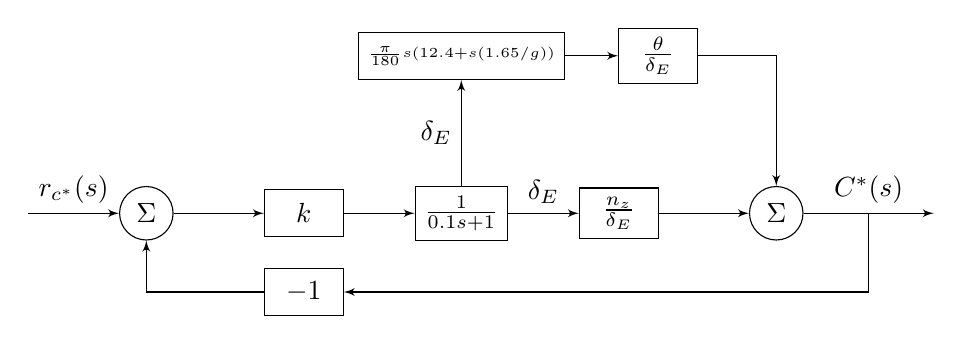
\begin{tikzpicture}[auto, node distance=2cm,>=latex']
            \node [input, name=input] {};
            \node [sum, right of=input, xshift=0.5cm] (sum1) {$\Sigma$};
            \node [block, right of=sum1] (controller) {$k$};
            \node [block, right of=controller] (actuator) {$\frac{1}{0.1s+1}$};
            \node [block, above of=actuator] (transfer) { $\scriptscriptstyle \frac{\pi}{180} s(12.4 + s(1.65/g))$};
            \node [block, right of=actuator] (plant) {$\frac{n_z}{\delta_E}$};
            \node [block, above of=plant, xshift=0.5cm] (plant2) {$\frac{\theta}{\delta_E}$};
            \node [sum, right of=plant, xshift=1cm] (sum2) {$\Sigma$};
            \node [output, right of=sum2] (output) {};
            \node [block, below of=controller, yshift=1cm] (feedback) {$-1$};
            \draw [draw,->] (input) -- node {$r_{c^*}(s)$} (sum1);
            \draw [->] (sum1) -- node {} (controller);
            \draw [->] (controller) -- node {} (actuator);
            \draw [->] (actuator) -- node {$\delta_E$} (plant);
            \draw [->] (actuator) -- node {$\delta_E$} (transfer);
            \draw [->] (sum2) -- node [name=y] {$C^*(s)$}(output);
            \draw [->] (y) |- node [above,pos=0.79] {} (feedback);
            \draw [->] (feedback) -| node  {} (sum1);
            \draw [->] (transfer) -- node {} (plant2);
            \draw [->] (plant) -- node {} (sum2);
            \draw [->] (plant2) -| node {} (sum2);
        \end{tikzpicture}
    \end{center}
    \caption{C* closed loop}
    \label{fig:cstar_diagram}
\end{figure}

To ensure the same denominator has identical poles for both pitch and normal acceleration transfer functions, the normal acceleration transfer function was taken from the representative \cite{rep}.

\begin{figure}[H]
    \centering
    \begin{subfigure}{0.45\textwidth}
        \centering
        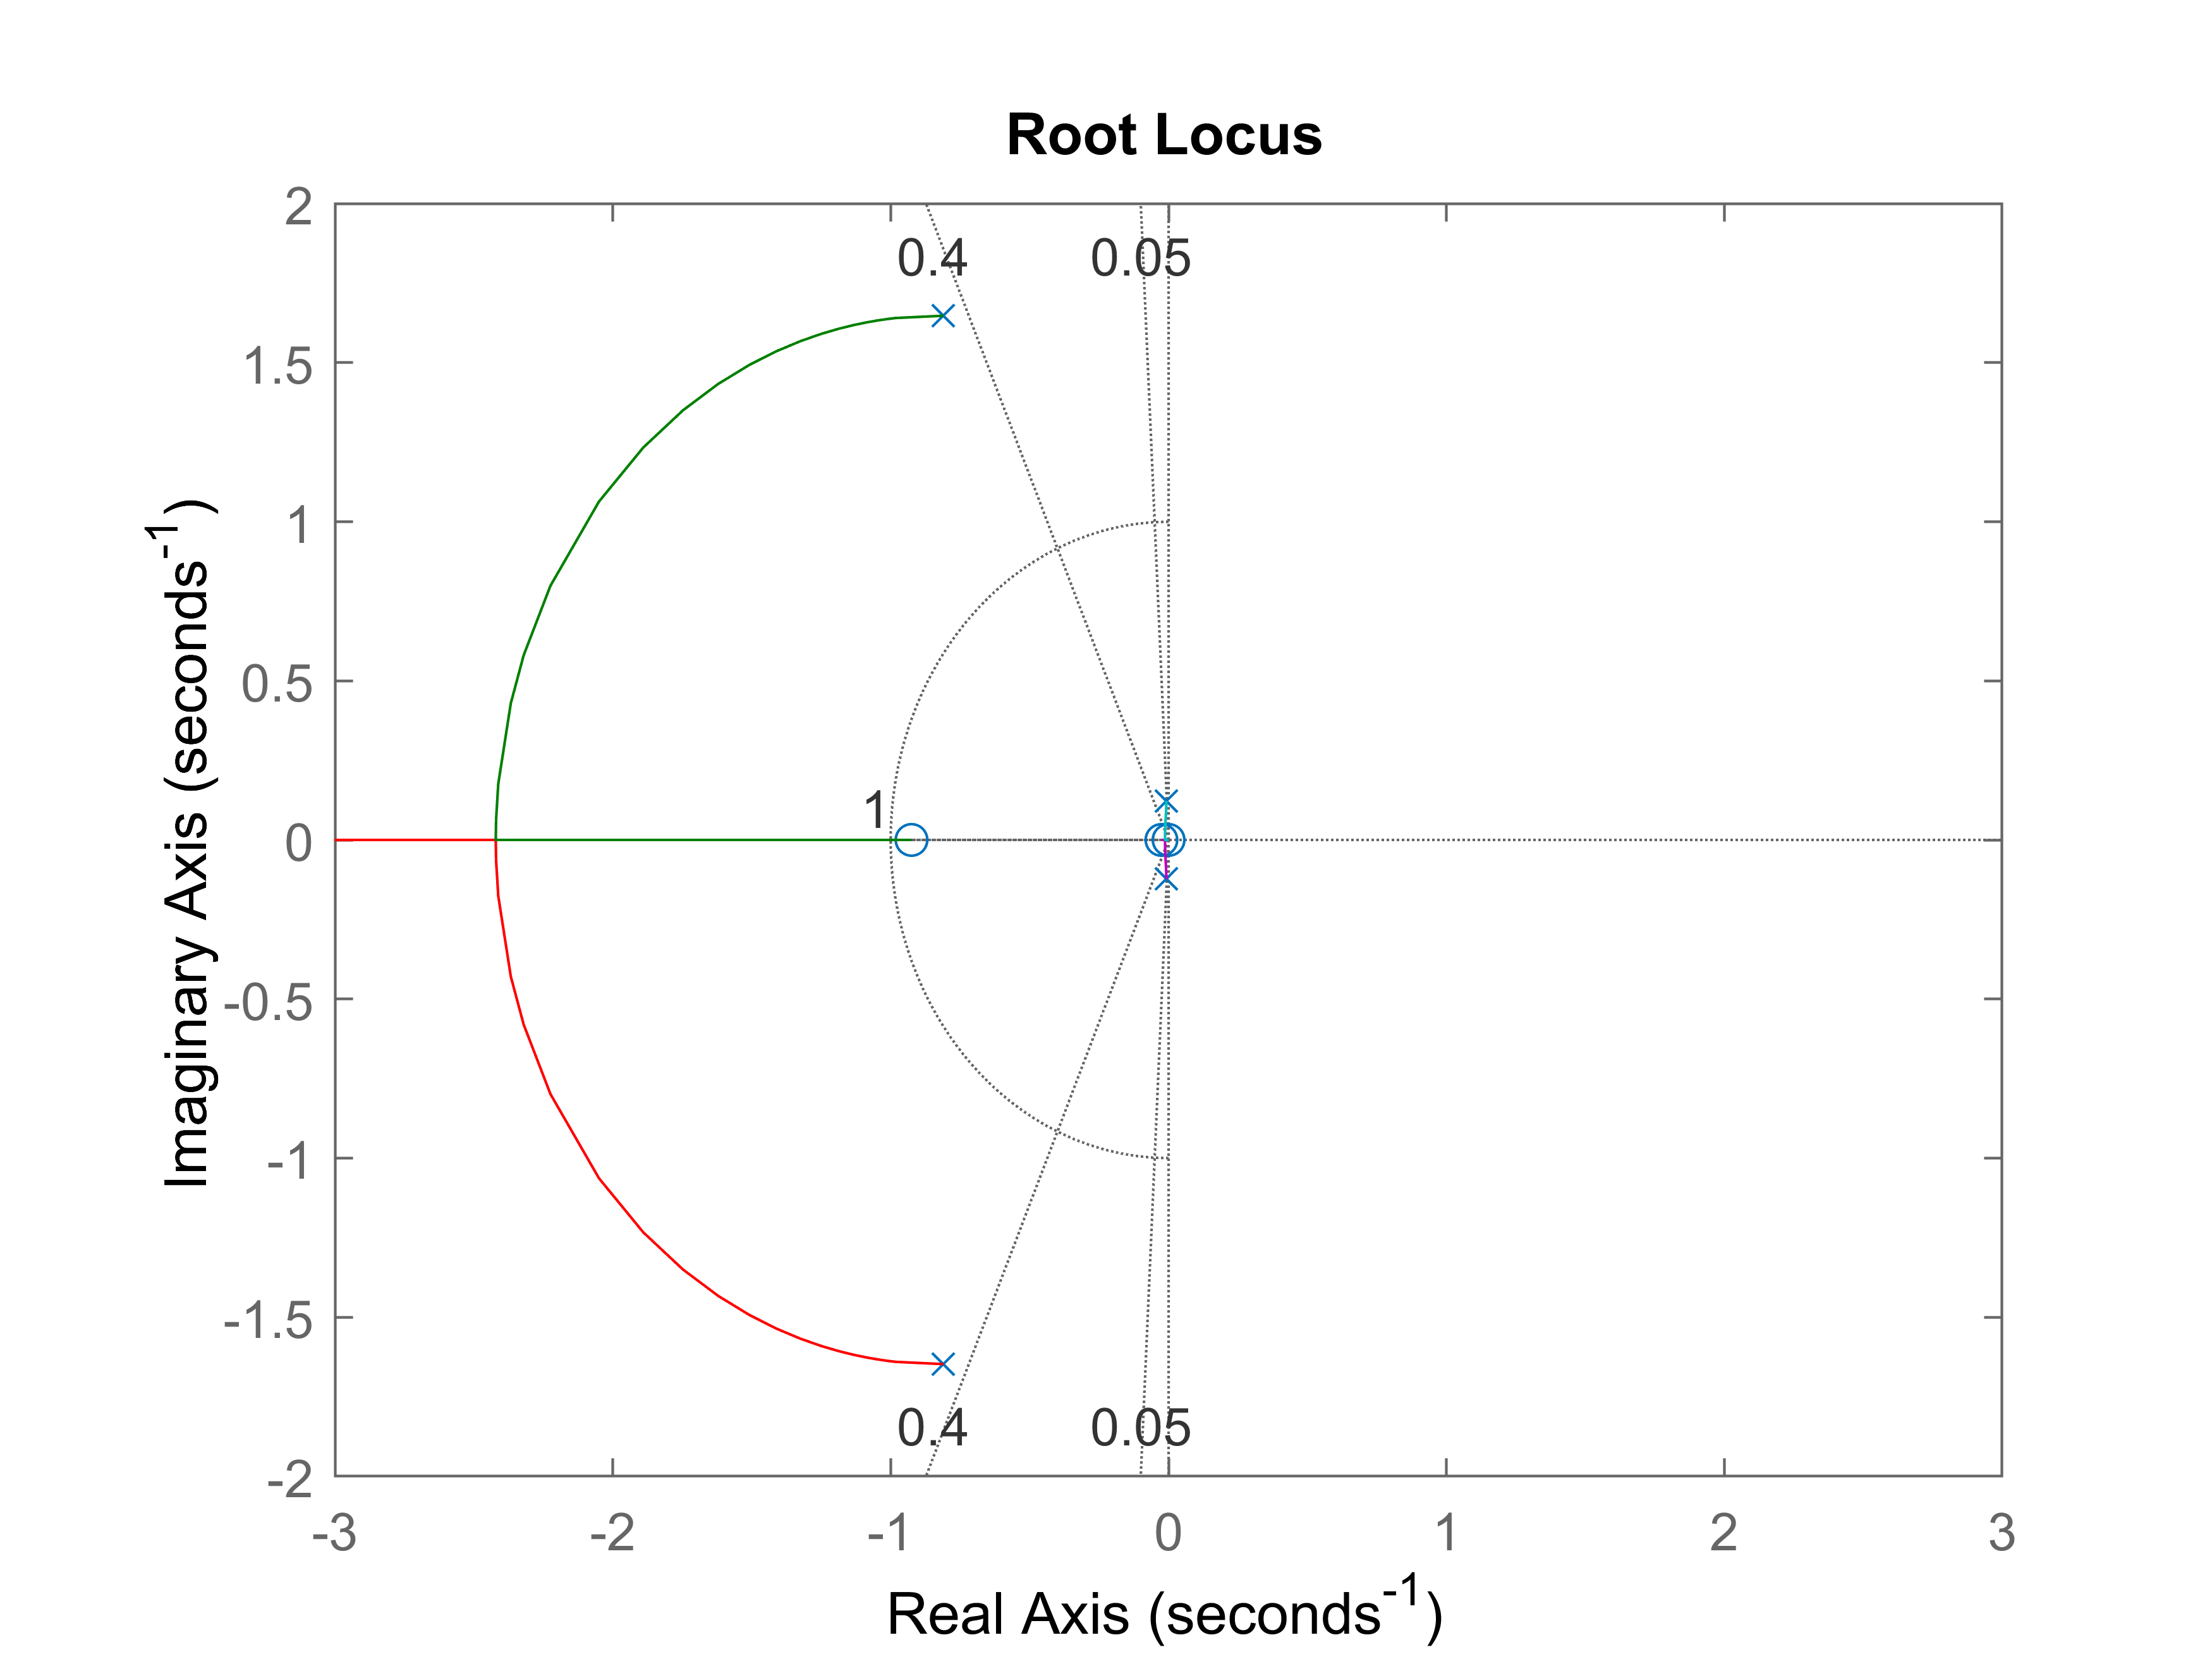
\includegraphics[width=0.99\textwidth]{figures/cstar_base_rlocus.png}
    \end{subfigure}
    \begin{subfigure}{0.45\textwidth}
        \centering
        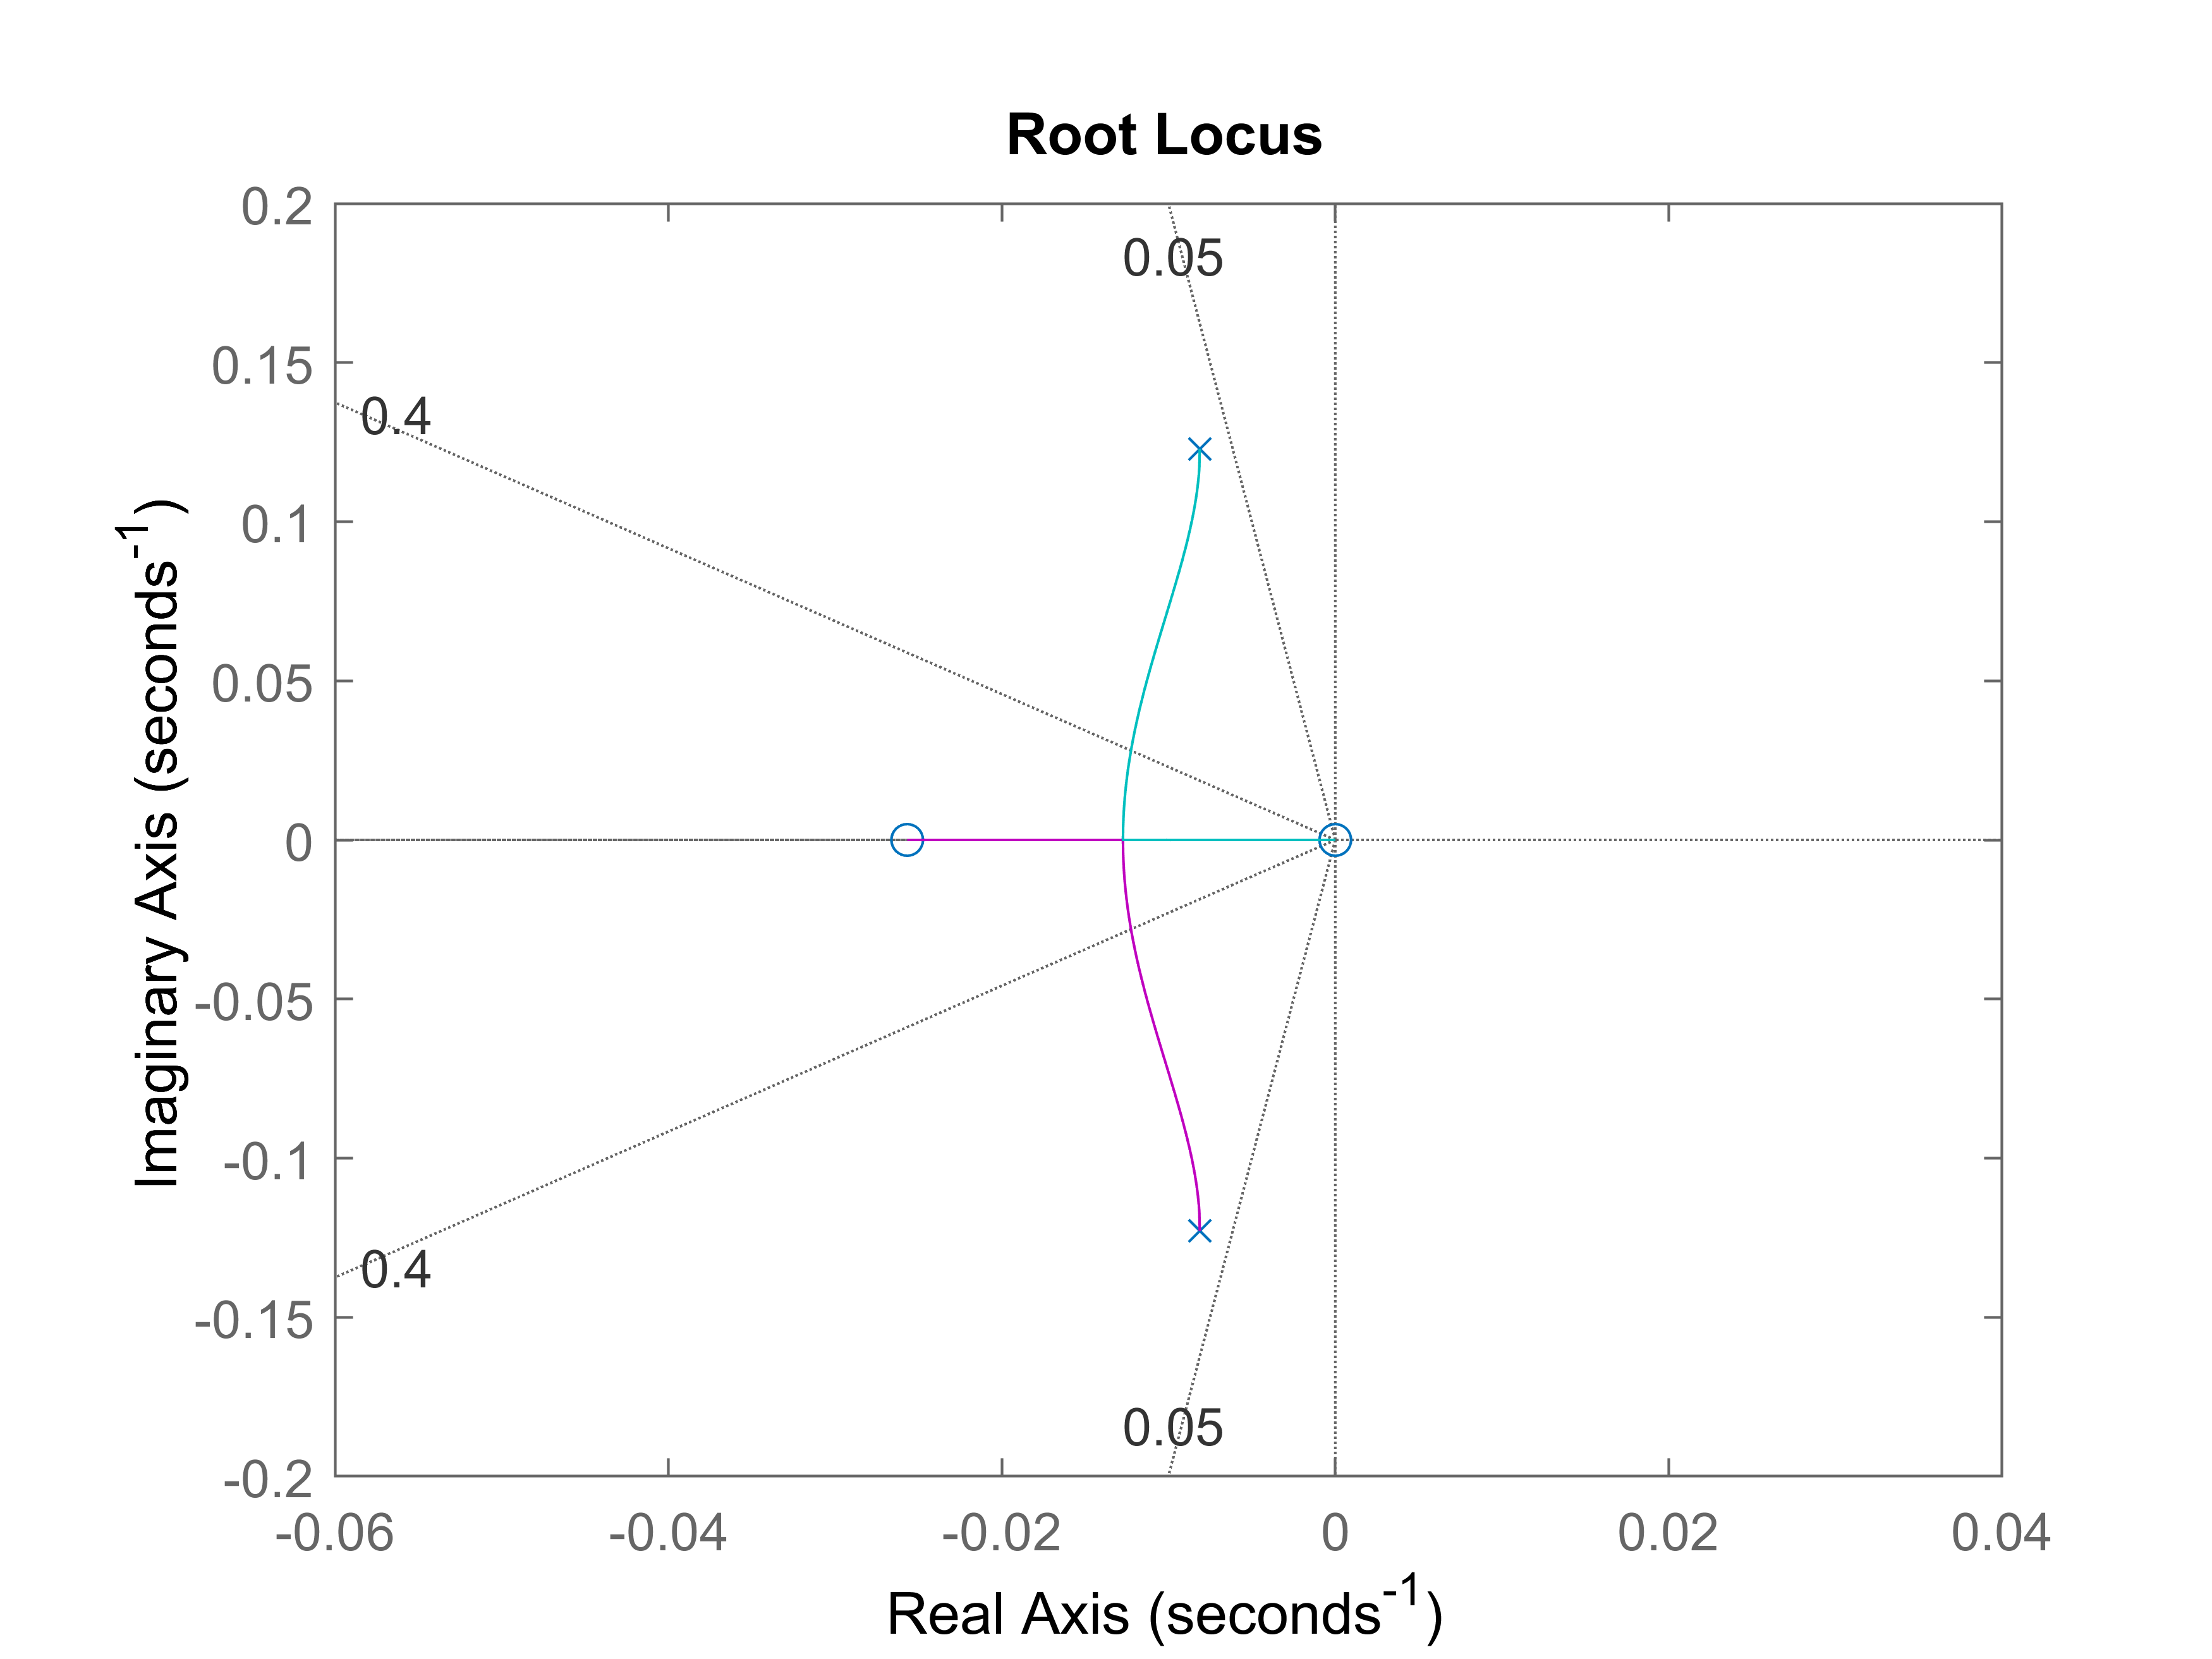
\includegraphics[width=0.99\textwidth]{figures/cstar_base_rlocus_zoomed.png}
    \end{subfigure}
    \caption{Root locus of $C^*$ control system with simple proportional controller.}
    \label{fig:cstar_base_rlocus}
\end{figure}

Figure \ref{fig:cstar_base_rlocus} shows the root locus of the $C^*$ control system with a simple proportional controller.
The addition of normal and pitch transfer functions with the same denominator caused a small numerical error in the denominator coefficients
which meant the same denominator could not be factored out.
This had the effect of adding additional poles and zeros very close to eachother such that their ratio was close to 1.
This can be seen in figure \ref{fig:matlab_numerical_errors}.
A different order of operation that avoided this was to sum the numerators before dividing by the denominator.
The requirements for the damping ratio for the chosen value of $k$ can be seen to be below the lines for the phugoid and SPO modes.

\begin{center}
     ( \texttt{rep\_elev\_norm\_num} $ + s(12.4 + 1.65s) \times $  \texttt{rep\_elev\_pitch\_num}) / \texttt{denominator};
\end{center}

\begin{figure}[H]
    \centering
    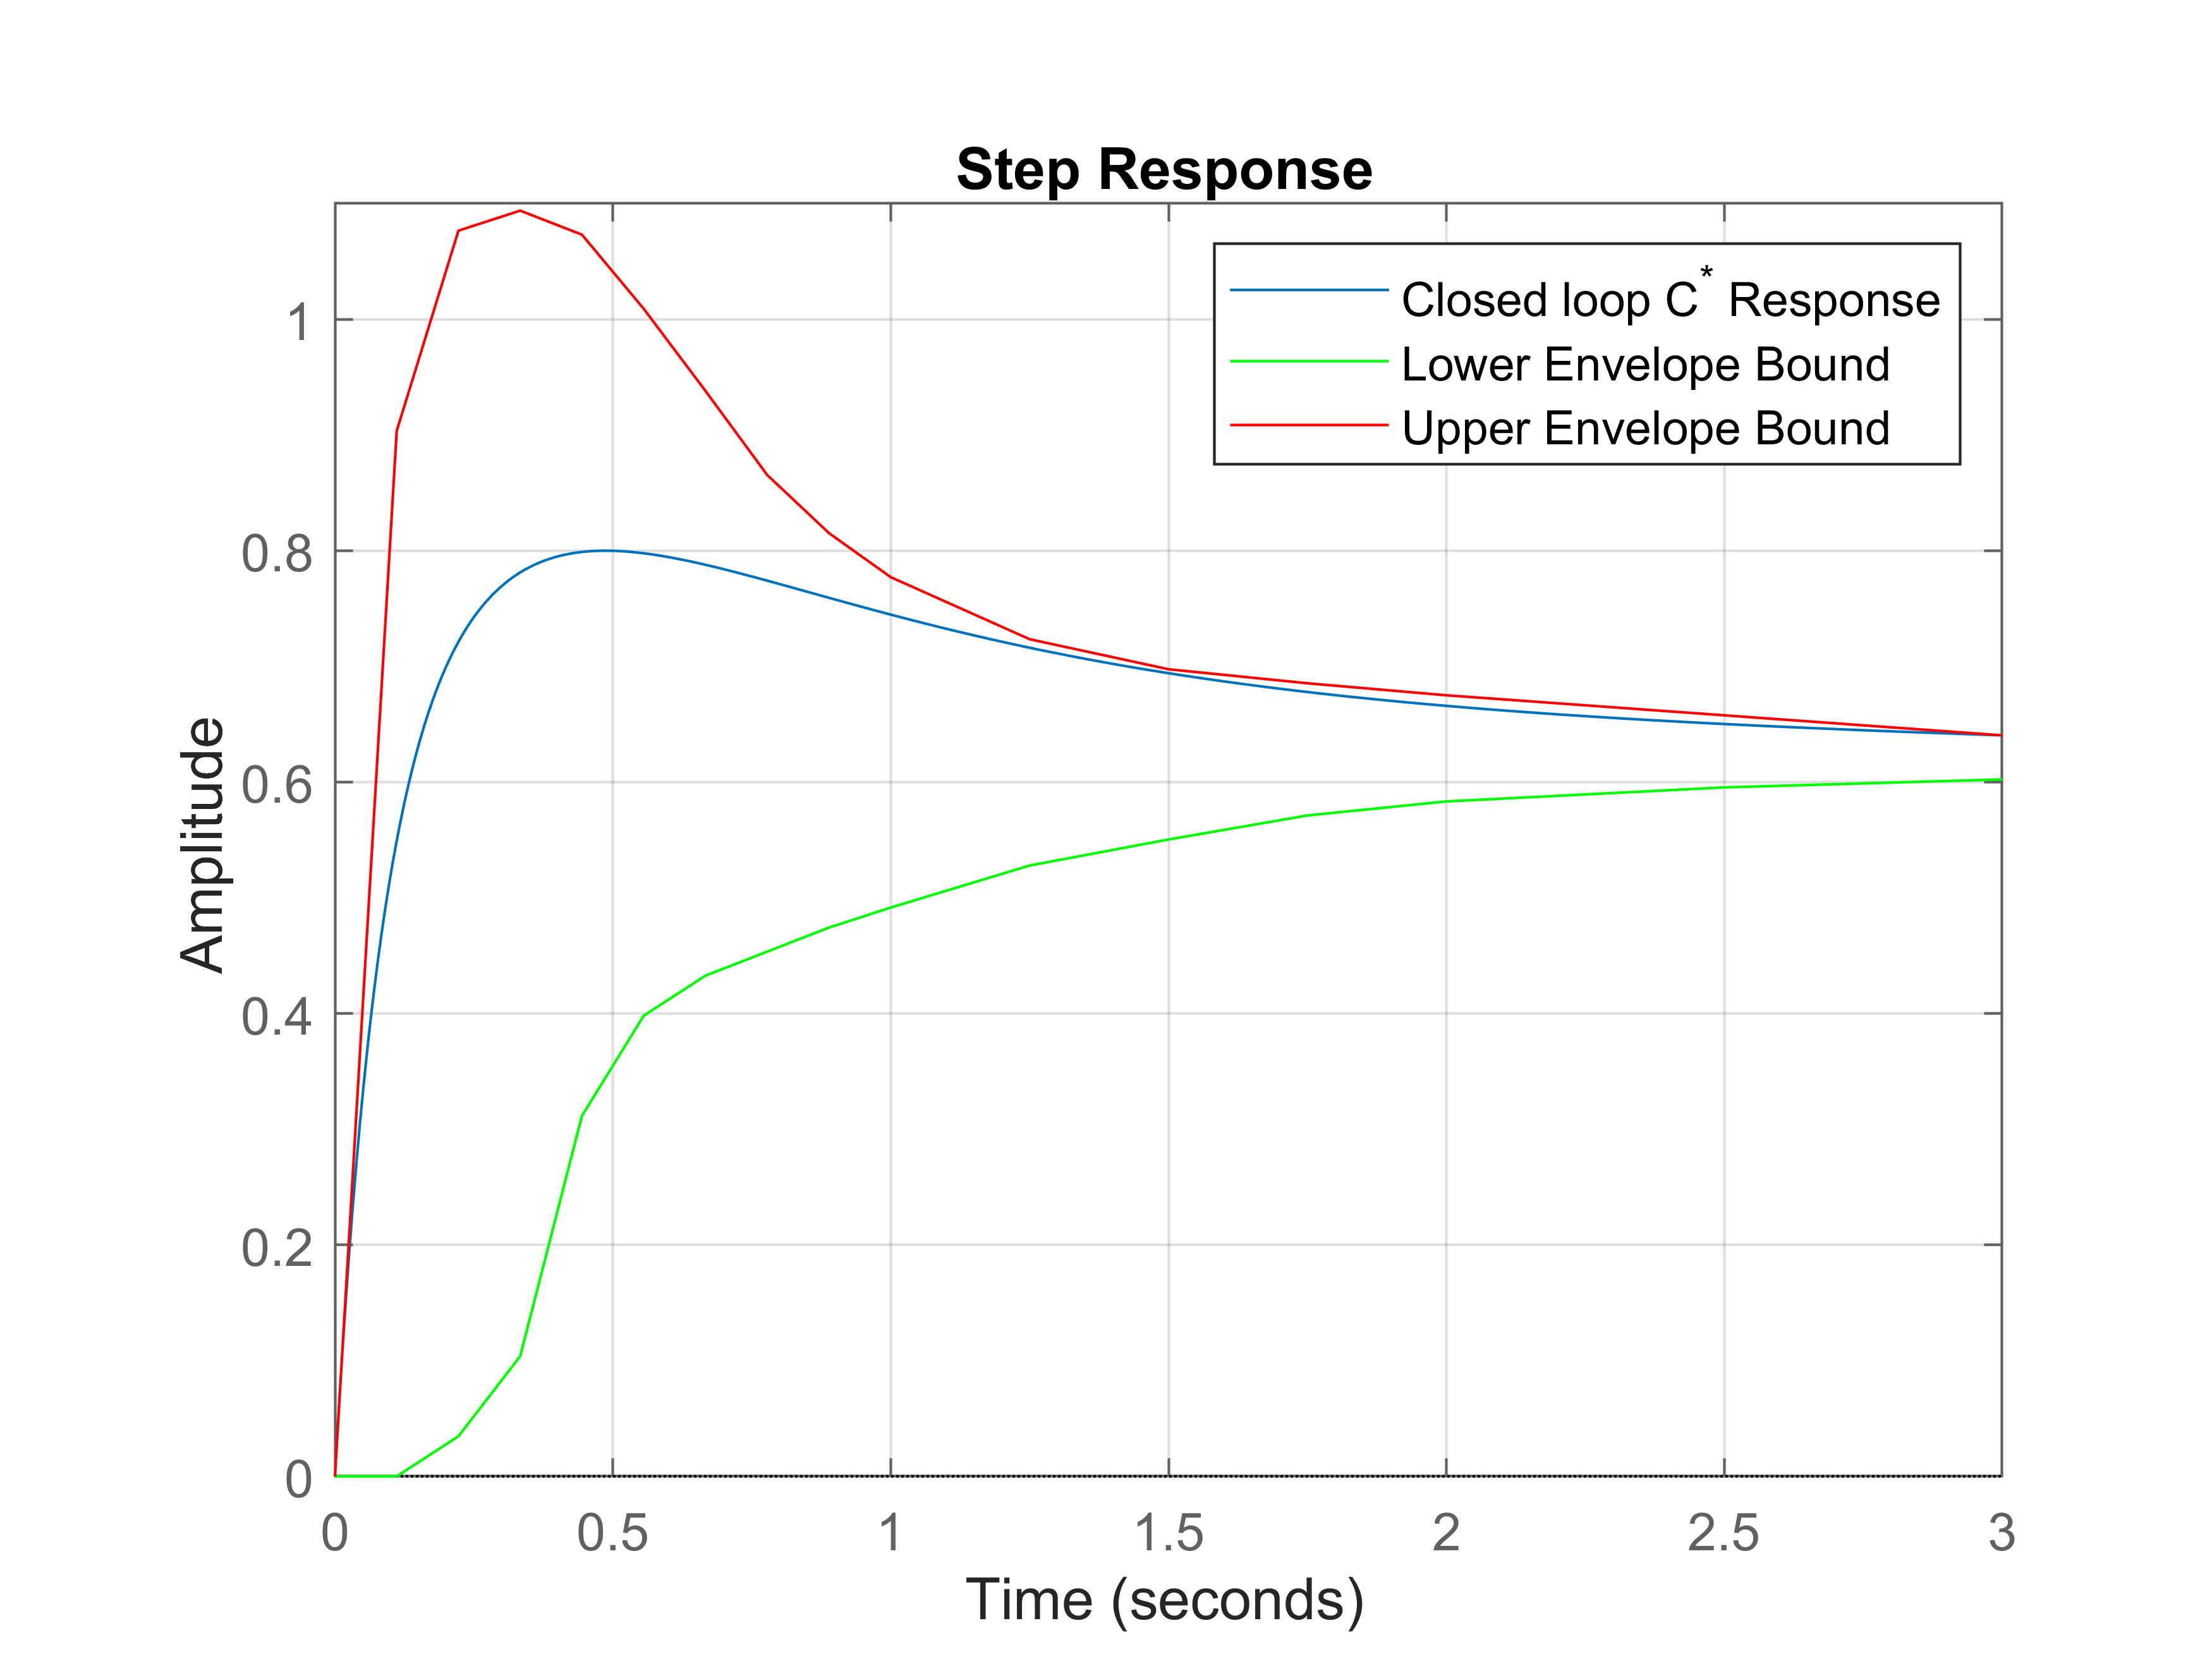
\includegraphics[width=0.6\textwidth]{figures/cstar_envelope_step.png}
    \caption{Step response of $C^*$ control system with simple proportional controller.}
    \label{fig:cstar_base_step}
\end{figure}

Figure \ref{fig:cstar_base_step} shows the step normalised response of the $C^*$ control system with a simple proportional controller.
A range of gains $4 > k > 50$ were found to fit the provided $C^*$ envelope, without any stability augmentation systems.
The value of gain $k=20$ was chosen as the peak was found to closely align with the envelope, providing the pilot with the best inertial feedback for comfort.
The additional distance from the envelope boundary also gives the control system robustness to uncertainty in the model and pilot experience.
A gain of $k=6$ corresponds to the neck of the balloon shaped locus where the damping of SPO was highest, this was not chosen however due to the slow response time of the system for this value.

\section{Improvements}

\begin{itemize}
    \item Representation of multiple input multiple output systems for coupled dynamics would allow for more accurate control system design at the loss of simple root locus analysis. LQR or H-infinity control could be used.
    \item Optimisation of controller parameters could be performed using a cost function based on the step response characteristics.
    \item Cross power spectral density analysis (Welch's method) would be significantly more robust to noise than the current method.
    This would allow for more accurate numerators to be fit to experimental data.
\end{itemize}


\section{Conclusion}

The importance of static aircraft stability and active flight control systems is discussed.
Static stability characteristics of the SAAB 340B were determined from experimental flight data.
Manouevre points of \dots
Modal analysis and transfer function fitting on frequency domain data was peformed to reconstruct the aircraft dynamics.
Discrepancies between the fitted and representative transfer functions were attributed to uncertainty in mode parameters and presence of noise in frequency domain data.
Robustness and performance requirements were defined for autopilot and augmented C* control systems.
The pitch displacement autopilot was found to require both integral and derivative terms to meet the requirements.
A tradeoff between the phugoid damping and SPO transience in the step response was identified and recommendations were made for the choice of gain value.
A proportional controller was found to meet requirements for the roll displacement autopilot, although its mentioned that a derivative term would improve performance.
The $C^*$ transfer function is derived and was found to meet requirements also with a simple proportional controller.
Finally, improvements to the analysis were suggested to better capture the dynamics of the aircraft and improve the robustness of the control system design.


\section{Appendix}

\begin{figure}[H]
    \centering
    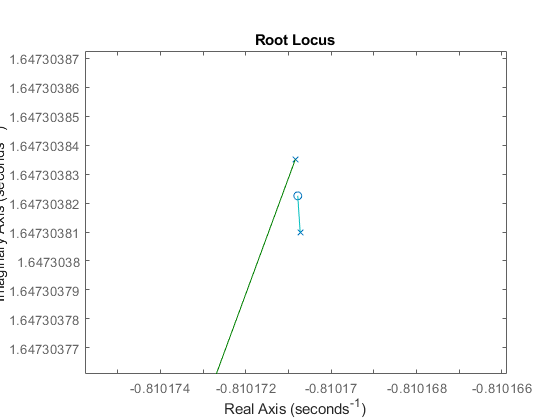
\includegraphics[width=0.6\textwidth]{figures/numerical_errors.png}
    \caption{Numerical errors from adding separate denominators}
    \label{fig:matlab_numerical_errors}
\end{figure}

\begin{figure}[H]
    \centering
    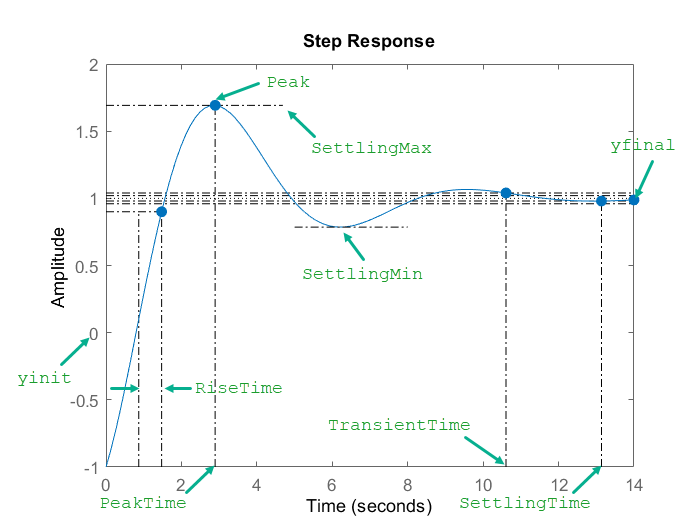
\includegraphics[width=0.6\textwidth]{figures/step-characteristics.png}
    \caption{Definition of step response characteristics \cite{matlab}.}
    \label{fig:matlab_step_chics}
\end{figure}

\begin{thebibliography}{9}

    \bibitem{handout}
    S. Place, A. Cooke
    \emph{Flight Experimental Methods: Course Handbook}
    Cranfield University,

    \bibitem{rep}
    University of Cambridge
    \emph{Representative Mode Parameters}

    \bibitem{autotune}
    A. S. McCormack and K. R. Godfrey
    \emph{Rule-Based Autotuning Based on Frequency Domain Identification}

    \bibitem{matlab}
    MATLAB
    \emph{Robust Performance Measure for Mu Synthesis}
    \texttt{https://uk.mathworks.com/help/robust/ug/measures-of-robust-performance.html}
    

\end{thebibliography}

\end{document}

